\documentclass[twoside]{book}

% Packages required by doxygen
\usepackage{fixltx2e}
\usepackage{calc}
\usepackage{doxygen}
\usepackage[export]{adjustbox} % also loads graphicx
\usepackage{graphicx}
\usepackage[utf8]{inputenc}
\usepackage{makeidx}
\usepackage{multicol}
\usepackage{multirow}
\PassOptionsToPackage{warn}{textcomp}
\usepackage{textcomp}
\usepackage[nointegrals]{wasysym}
\usepackage[table]{xcolor}

% Font selection
\usepackage[T1]{fontenc}
\usepackage[scaled=.90]{helvet}
\usepackage{courier}
\usepackage{amssymb}
\usepackage{sectsty}
\renewcommand{\familydefault}{\sfdefault}
\allsectionsfont{%
  \fontseries{bc}\selectfont%
  \color{darkgray}%
}
\renewcommand{\DoxyLabelFont}{%
  \fontseries{bc}\selectfont%
  \color{darkgray}%
}
\newcommand{\+}{\discretionary{\mbox{\scriptsize$\hookleftarrow$}}{}{}}

% Page & text layout
\usepackage{geometry}
\geometry{%
  a4paper,%
  top=2.5cm,%
  bottom=2.5cm,%
  left=2.5cm,%
  right=2.5cm%
}
\tolerance=750
\hfuzz=15pt
\hbadness=750
\setlength{\emergencystretch}{15pt}
\setlength{\parindent}{0cm}
\setlength{\parskip}{0.2cm}
\makeatletter
\renewcommand{\paragraph}{%
  \@startsection{paragraph}{4}{0ex}{-1.0ex}{1.0ex}{%
    \normalfont\normalsize\bfseries\SS@parafont%
  }%
}
\renewcommand{\subparagraph}{%
  \@startsection{subparagraph}{5}{0ex}{-1.0ex}{1.0ex}{%
    \normalfont\normalsize\bfseries\SS@subparafont%
  }%
}
\makeatother

% Headers & footers
\usepackage{fancyhdr}
\pagestyle{fancyplain}
\fancyhead[LE]{\fancyplain{}{\bfseries\thepage}}
\fancyhead[CE]{\fancyplain{}{}}
\fancyhead[RE]{\fancyplain{}{\bfseries\leftmark}}
\fancyhead[LO]{\fancyplain{}{\bfseries\rightmark}}
\fancyhead[CO]{\fancyplain{}{}}
\fancyhead[RO]{\fancyplain{}{\bfseries\thepage}}
\fancyfoot[LE]{\fancyplain{}{}}
\fancyfoot[CE]{\fancyplain{}{}}
\fancyfoot[RE]{\fancyplain{}{\bfseries\scriptsize Generated on Wed Mar 18 2015 15\+:38\+:24 for im\+Calculator by Doxygen }}
\fancyfoot[LO]{\fancyplain{}{\bfseries\scriptsize Generated on Wed Mar 18 2015 15\+:38\+:24 for im\+Calculator by Doxygen }}
\fancyfoot[CO]{\fancyplain{}{}}
\fancyfoot[RO]{\fancyplain{}{}}
\renewcommand{\footrulewidth}{0.4pt}
\renewcommand{\chaptermark}[1]{%
  \markboth{#1}{}%
}
\renewcommand{\sectionmark}[1]{%
  \markright{\thesection\ #1}%
}

% Indices & bibliography
\usepackage{natbib}
\usepackage[titles]{tocloft}
\setcounter{tocdepth}{3}
\setcounter{secnumdepth}{5}
\makeindex

% Hyperlinks (required, but should be loaded last)
\usepackage{ifpdf}
\ifpdf
  \usepackage[pdftex,pagebackref=true]{hyperref}
\else
  \usepackage[ps2pdf,pagebackref=true]{hyperref}
\fi
\hypersetup{%
  colorlinks=true,%
  linkcolor=blue,%
  citecolor=blue,%
  unicode%
}

% Custom commands
\newcommand{\clearemptydoublepage}{%
  \newpage{\pagestyle{empty}\cleardoublepage}%
}


%===== C O N T E N T S =====

\begin{document}

% Titlepage & ToC
\hypersetup{pageanchor=false,
             bookmarks=true,
             bookmarksnumbered=true,
             pdfencoding=unicode
            }
\pagenumbering{roman}
\begin{titlepage}
\vspace*{7cm}
\begin{center}%
{\Large im\+Calculator \\[1ex]\large 1.\+0 }\\
\vspace*{1cm}
{\large Generated by Doxygen 1.8.9.1}\\
\vspace*{0.5cm}
{\small Wed Mar 18 2015 15:38:24}\\
\end{center}
\end{titlepage}
\clearemptydoublepage
\tableofcontents
\clearemptydoublepage
\pagenumbering{arabic}
\hypersetup{pageanchor=true}

%--- Begin generated contents ---
\chapter{Hierarchical Index}
\section{Class Hierarchy}
This inheritance list is sorted roughly, but not completely, alphabetically\+:\begin{DoxyCompactList}
\item \contentsline{section}{Class\+Controller}{\pageref{class_class_controller}}{}
\item \contentsline{section}{Equation\+Exception}{\pageref{class_equation_exception}}{}
\item \contentsline{section}{Expression}{\pageref{class_expression}}{}
\begin{DoxyCompactList}
\item \contentsline{section}{Equation}{\pageref{class_equation}}{}
\end{DoxyCompactList}
\item \contentsline{section}{Extension}{\pageref{class_extension}}{}
\item \contentsline{section}{list$<$ T $>$}{\pageref{classlist}}{}
\item \contentsline{section}{list$<$ Token $\ast$ $>$}{\pageref{classlist}}{}
\item \contentsline{section}{Log}{\pageref{class_log}}{}
\item \contentsline{section}{Logger}{\pageref{class_logger}}{}
\item \contentsline{section}{Reader}{\pageref{class_reader}}{}
\item \contentsline{section}{Saver}{\pageref{class_saver}}{}
\item \contentsline{section}{stack$<$ T $>$}{\pageref{classstack}}{}
\item \contentsline{section}{stack$<$ Token $\ast$ $>$}{\pageref{classstack}}{}
\item \contentsline{section}{Token}{\pageref{class_token}}{}
\begin{DoxyCompactList}
\item \contentsline{section}{Logic}{\pageref{class_logic}}{}
\item \contentsline{section}{Number}{\pageref{class_number}}{}
\begin{DoxyCompactList}
\item \contentsline{section}{Number\+Arab}{\pageref{class_number_arab}}{}
\item \contentsline{section}{Number\+Romawi}{\pageref{class_number_romawi}}{}
\end{DoxyCompactList}
\end{DoxyCompactList}
\item \contentsline{section}{vector$<$ T $>$}{\pageref{classvector}}{}
\item \contentsline{section}{vector$<$ Log $>$}{\pageref{classvector}}{}
\end{DoxyCompactList}

\chapter{Class Index}
\section{Class List}
Here are the classes, structs, unions and interfaces with brief descriptions\+:\begin{DoxyCompactList}
\item\contentsline{section}{\hyperlink{class_class_controller}{Class\+Controller} }{\pageref{class_class_controller}}{}
\item\contentsline{section}{\hyperlink{class_equation}{Equation} }{\pageref{class_equation}}{}
\item\contentsline{section}{\hyperlink{class_equation_exception}{Equation\+Exception} }{\pageref{class_equation_exception}}{}
\item\contentsline{section}{\hyperlink{class_expression}{Expression} }{\pageref{class_expression}}{}
\item\contentsline{section}{\hyperlink{class_extension}{Extension} \\*Kelas \hyperlink{class_extension}{Extension} berisi konstanta yang dibutuhkan dalam program }{\pageref{class_extension}}{}
\item\contentsline{section}{\hyperlink{classlist}{list$<$ T $>$} }{\pageref{classlist}}{}
\item\contentsline{section}{\hyperlink{class_log}{Log} \\*Kelas \hyperlink{class_log}{Log} adalah abstract data type untuk log command }{\pageref{class_log}}{}
\item\contentsline{section}{\hyperlink{class_logger}{Logger} \\*Kelas \hyperlink{class_log}{Log} adalah abstract data type untuk log command }{\pageref{class_logger}}{}
\item\contentsline{section}{\hyperlink{class_logic}{Logic} }{\pageref{class_logic}}{}
\item\contentsline{section}{\hyperlink{class_number}{Number} }{\pageref{class_number}}{}
\item\contentsline{section}{\hyperlink{class_number_arab}{Number\+Arab} }{\pageref{class_number_arab}}{}
\item\contentsline{section}{\hyperlink{class_number_romawi}{Number\+Romawi} }{\pageref{class_number_romawi}}{}
\item\contentsline{section}{\hyperlink{class_reader}{Reader} \\*Kelas \hyperlink{class_reader}{Reader} bertugas menerima input dari user kemudian mengkategorikan input tersebut termasuk command atau ekspresi }{\pageref{class_reader}}{}
\item\contentsline{section}{\hyperlink{class_saver}{Saver} \\*Kelas \hyperlink{class_class_controller}{Class\+Controller} bertugas untuk mengatur kehidupan dan kematian kelas-\/kelas lain }{\pageref{class_saver}}{}
\item\contentsline{section}{\hyperlink{classstack}{stack$<$ T $>$} }{\pageref{classstack}}{}
\item\contentsline{section}{\hyperlink{class_token}{Token} }{\pageref{class_token}}{}
\item\contentsline{section}{\hyperlink{classvector}{vector$<$ T $>$} \\*Vector adalah implementasi vector yang ekuivalen vector S\+T\+L C++ }{\pageref{classvector}}{}
\end{DoxyCompactList}

\chapter{Class Documentation}
\hypertarget{class_class_controller}{}\section{Class\+Controller Class Reference}
\label{class_class_controller}\index{Class\+Controller@{Class\+Controller}}
\subsection*{Public Member Functions}
\begin{DoxyCompactItemize}
\item 
\hypertarget{class_class_controller_aabaaed00c4700f5aaa10012a0616e516}{}\hyperlink{class_class_controller_aabaaed00c4700f5aaa10012a0616e516}{Class\+Controller} ()\label{class_class_controller_aabaaed00c4700f5aaa10012a0616e516}

\begin{DoxyCompactList}\small\item\em Konstruktor kelas \hyperlink{class_class_controller}{Class\+Controller}. \end{DoxyCompactList}\item 
\hyperlink{class_class_controller_a2bfe283911ba627fb346aa9a2e149fd1}{Class\+Controller} (const \hyperlink{class_class_controller}{Class\+Controller} \&)
\begin{DoxyCompactList}\small\item\em Copy Constructor kelas \hyperlink{class_class_controller}{Class\+Controller} dengan parameter. \end{DoxyCompactList}\item 
\hypertarget{class_class_controller_ab8f18f58ffb5cfc71da0d5a28ac1b657}{}\hyperlink{class_class_controller}{Class\+Controller} \& \hyperlink{class_class_controller_ab8f18f58ffb5cfc71da0d5a28ac1b657}{operator=} (const \hyperlink{class_class_controller}{Class\+Controller} \&)\label{class_class_controller_ab8f18f58ffb5cfc71da0d5a28ac1b657}

\begin{DoxyCompactList}\small\item\em Operator assignment kelas \hyperlink{class_class_controller}{Class\+Controller}. \end{DoxyCompactList}\item 
\hypertarget{class_class_controller_ae511f4053f0dd4a11805482f39e576ca}{}\hyperlink{class_class_controller_ae511f4053f0dd4a11805482f39e576ca}{$\sim$\+Class\+Controller} ()\label{class_class_controller_ae511f4053f0dd4a11805482f39e576ca}

\begin{DoxyCompactList}\small\item\em Destruktor kelas \hyperlink{class_class_controller}{Class\+Controller}. \end{DoxyCompactList}\item 
void \hyperlink{class_class_controller_a06cb940d9bfa3a4ec30dcd88c05c2e52}{Execute\+Expression} (string \&)
\begin{DoxyCompactList}\small\item\em Mengeksekusi ekspresi yang dimasukkan oleh user. \end{DoxyCompactList}\item 
void \hyperlink{class_class_controller_a8bee544a3a5f0de7863800aa0ef093f0}{Execute\+Command} (string)
\begin{DoxyCompactList}\small\item\em Mengeksekusi command yang dimasukkan oleh user. \end{DoxyCompactList}\item 
void \hyperlink{class_class_controller_a9caf153dbff2f0be07809b50d52b782f}{Undo} (int)
\begin{DoxyCompactList}\small\item\em Mengembalikan perintah yang telah dimasukkan user. \end{DoxyCompactList}\item 
void \hyperlink{class_class_controller_a4f77c68f3f4418d364aab3eb5cecf26a}{Redo} (int)
\begin{DoxyCompactList}\small\item\em Mengembalikan perintah yang telah di-\/undo user. \end{DoxyCompactList}\item 
void \hyperlink{class_class_controller_a95d115cd68bc470b0c5aefa7aaa33b38}{Set\+Expression\+Mode} (int)
\begin{DoxyCompactList}\small\item\em Mengubah mode ekspresi (prefiks -\/ infiks -\/ postfiks) \end{DoxyCompactList}\item 
void \hyperlink{class_class_controller_aa983bd9a5b63d3d19aa0374d39dda9fc}{Set\+Equation\+Mode} (int)
\begin{DoxyCompactList}\small\item\em Mengubah mode equation (bilangan -\/ logika) \end{DoxyCompactList}\item 
void \hyperlink{class_class_controller_a7522169d820cd667954776ad8dfdba40}{Set\+Number\+Mode} (int)
\begin{DoxyCompactList}\small\item\em Mengubah mode number (romawi -\/ arab) \end{DoxyCompactList}\item 
\hypertarget{class_class_controller_a9e249c8cca0d1f9f55d39050674f9641}{}void \hyperlink{class_class_controller_a9e249c8cca0d1f9f55d39050674f9641}{Reset\+Setting} ()\label{class_class_controller_a9e249c8cca0d1f9f55d39050674f9641}

\begin{DoxyCompactList}\small\item\em Mengembalikan setting ke mode default. \end{DoxyCompactList}\item 
void \hyperlink{class_class_controller_a1ac2d697860226759069791ff937220a}{Show\+Mem} (int)
\begin{DoxyCompactList}\small\item\em Menampilkan n perintah terakhir yang dimasukkan user. \end{DoxyCompactList}\item 
\hypertarget{class_class_controller_a26931f9359bf51872585e1bbfba2b881}{}void \hyperlink{class_class_controller_a26931f9359bf51872585e1bbfba2b881}{Show\+Mem\+All} ()\label{class_class_controller_a26931f9359bf51872585e1bbfba2b881}

\begin{DoxyCompactList}\small\item\em Menampilkan semua perintah yang dimasukkan user. \end{DoxyCompactList}\item 
\hypertarget{class_class_controller_ac189afe69eef22e5602ada767001cd75}{}void \hyperlink{class_class_controller_ac189afe69eef22e5602ada767001cd75}{Help} ()\label{class_class_controller_ac189afe69eef22e5602ada767001cd75}

\begin{DoxyCompactList}\small\item\em Menampilkan \textquotesingle{}help\textquotesingle{} yang berisi daftar command yang berlaku dalam program. \end{DoxyCompactList}\item 
\hypertarget{class_class_controller_ac186b106003efe4d502d9630653e84b3}{}void \hyperlink{class_class_controller_ac186b106003efe4d502d9630653e84b3}{View\+Setting} ()\label{class_class_controller_ac186b106003efe4d502d9630653e84b3}

\begin{DoxyCompactList}\small\item\em Menampilkan mode setting terkini. \end{DoxyCompactList}\end{DoxyCompactItemize}


\subsection{Constructor \& Destructor Documentation}
\hypertarget{class_class_controller_a2bfe283911ba627fb346aa9a2e149fd1}{}\index{Class\+Controller@{Class\+Controller}!Class\+Controller@{Class\+Controller}}
\index{Class\+Controller@{Class\+Controller}!Class\+Controller@{Class\+Controller}}
\subsubsection[{Class\+Controller}]{\setlength{\rightskip}{0pt plus 5cm}Class\+Controller\+::\+Class\+Controller (
\begin{DoxyParamCaption}
\item[{const {\bf Class\+Controller} \&}]{man}
\end{DoxyParamCaption}
)}\label{class_class_controller_a2bfe283911ba627fb346aa9a2e149fd1}


Copy Constructor kelas \hyperlink{class_class_controller}{Class\+Controller} dengan parameter. 


\begin{DoxyParams}{Parameters}
{\em \hyperlink{class_class_controller}{Class\+Controller}} & yang akan di-\/copy. \\
\hline
\end{DoxyParams}


\subsection{Member Function Documentation}
\hypertarget{class_class_controller_a8bee544a3a5f0de7863800aa0ef093f0}{}\index{Class\+Controller@{Class\+Controller}!Execute\+Command@{Execute\+Command}}
\index{Execute\+Command@{Execute\+Command}!Class\+Controller@{Class\+Controller}}
\subsubsection[{Execute\+Command}]{\setlength{\rightskip}{0pt plus 5cm}void Class\+Controller\+::\+Execute\+Command (
\begin{DoxyParamCaption}
\item[{string}]{buffer}
\end{DoxyParamCaption}
)}\label{class_class_controller_a8bee544a3a5f0de7863800aa0ef093f0}


Mengeksekusi command yang dimasukkan oleh user. 


\begin{DoxyParams}{Parameters}
{\em string} & -\/ masukan string command yang akan dieksekusi. \\
\hline
\end{DoxyParams}
\hypertarget{class_class_controller_a06cb940d9bfa3a4ec30dcd88c05c2e52}{}\index{Class\+Controller@{Class\+Controller}!Execute\+Expression@{Execute\+Expression}}
\index{Execute\+Expression@{Execute\+Expression}!Class\+Controller@{Class\+Controller}}
\subsubsection[{Execute\+Expression}]{\setlength{\rightskip}{0pt plus 5cm}void Class\+Controller\+::\+Execute\+Expression (
\begin{DoxyParamCaption}
\item[{string \&}]{buffer}
\end{DoxyParamCaption}
)}\label{class_class_controller_a06cb940d9bfa3a4ec30dcd88c05c2e52}


Mengeksekusi ekspresi yang dimasukkan oleh user. 


\begin{DoxyParams}{Parameters}
{\em string} & -\/ masukan string ekspresi yang akan dieksekusi. \\
\hline
\end{DoxyParams}
\hypertarget{class_class_controller_a4f77c68f3f4418d364aab3eb5cecf26a}{}\index{Class\+Controller@{Class\+Controller}!Redo@{Redo}}
\index{Redo@{Redo}!Class\+Controller@{Class\+Controller}}
\subsubsection[{Redo}]{\setlength{\rightskip}{0pt plus 5cm}void Class\+Controller\+::\+Redo (
\begin{DoxyParamCaption}
\item[{int}]{n}
\end{DoxyParamCaption}
)}\label{class_class_controller_a4f77c68f3f4418d364aab3eb5cecf26a}


Mengembalikan perintah yang telah di-\/undo user. 


\begin{DoxyParams}{Parameters}
{\em int} & -\/ banyak perintah. \\
\hline
\end{DoxyParams}
\hypertarget{class_class_controller_aa983bd9a5b63d3d19aa0374d39dda9fc}{}\index{Class\+Controller@{Class\+Controller}!Set\+Equation\+Mode@{Set\+Equation\+Mode}}
\index{Set\+Equation\+Mode@{Set\+Equation\+Mode}!Class\+Controller@{Class\+Controller}}
\subsubsection[{Set\+Equation\+Mode}]{\setlength{\rightskip}{0pt plus 5cm}void Class\+Controller\+::\+Set\+Equation\+Mode (
\begin{DoxyParamCaption}
\item[{int}]{equation\+Mode}
\end{DoxyParamCaption}
)}\label{class_class_controller_aa983bd9a5b63d3d19aa0374d39dda9fc}


Mengubah mode equation (bilangan -\/ logika) 


\begin{DoxyParams}{Parameters}
{\em int} & -\/ nomor setting (ada di kelas \hyperlink{class_extension}{Extension}). \\
\hline
\end{DoxyParams}
\hypertarget{class_class_controller_a95d115cd68bc470b0c5aefa7aaa33b38}{}\index{Class\+Controller@{Class\+Controller}!Set\+Expression\+Mode@{Set\+Expression\+Mode}}
\index{Set\+Expression\+Mode@{Set\+Expression\+Mode}!Class\+Controller@{Class\+Controller}}
\subsubsection[{Set\+Expression\+Mode}]{\setlength{\rightskip}{0pt plus 5cm}void Class\+Controller\+::\+Set\+Expression\+Mode (
\begin{DoxyParamCaption}
\item[{int}]{expression\+Mode}
\end{DoxyParamCaption}
)}\label{class_class_controller_a95d115cd68bc470b0c5aefa7aaa33b38}


Mengubah mode ekspresi (prefiks -\/ infiks -\/ postfiks) 


\begin{DoxyParams}{Parameters}
{\em int} & -\/ nomor setting (ada di kelas \hyperlink{class_extension}{Extension}). \\
\hline
\end{DoxyParams}
\hypertarget{class_class_controller_a7522169d820cd667954776ad8dfdba40}{}\index{Class\+Controller@{Class\+Controller}!Set\+Number\+Mode@{Set\+Number\+Mode}}
\index{Set\+Number\+Mode@{Set\+Number\+Mode}!Class\+Controller@{Class\+Controller}}
\subsubsection[{Set\+Number\+Mode}]{\setlength{\rightskip}{0pt plus 5cm}void Class\+Controller\+::\+Set\+Number\+Mode (
\begin{DoxyParamCaption}
\item[{int}]{number\+Mode}
\end{DoxyParamCaption}
)}\label{class_class_controller_a7522169d820cd667954776ad8dfdba40}


Mengubah mode number (romawi -\/ arab) 


\begin{DoxyParams}{Parameters}
{\em int} & -\/ nomor setting (ada di kelas \hyperlink{class_extension}{Extension}). \\
\hline
\end{DoxyParams}
\hypertarget{class_class_controller_a1ac2d697860226759069791ff937220a}{}\index{Class\+Controller@{Class\+Controller}!Show\+Mem@{Show\+Mem}}
\index{Show\+Mem@{Show\+Mem}!Class\+Controller@{Class\+Controller}}
\subsubsection[{Show\+Mem}]{\setlength{\rightskip}{0pt plus 5cm}void Class\+Controller\+::\+Show\+Mem (
\begin{DoxyParamCaption}
\item[{int}]{n}
\end{DoxyParamCaption}
)}\label{class_class_controller_a1ac2d697860226759069791ff937220a}


Menampilkan n perintah terakhir yang dimasukkan user. 


\begin{DoxyParams}{Parameters}
{\em n} & -\/ int. Banyak perintah. \\
\hline
\end{DoxyParams}
\hypertarget{class_class_controller_a9caf153dbff2f0be07809b50d52b782f}{}\index{Class\+Controller@{Class\+Controller}!Undo@{Undo}}
\index{Undo@{Undo}!Class\+Controller@{Class\+Controller}}
\subsubsection[{Undo}]{\setlength{\rightskip}{0pt plus 5cm}void Class\+Controller\+::\+Undo (
\begin{DoxyParamCaption}
\item[{int}]{n}
\end{DoxyParamCaption}
)}\label{class_class_controller_a9caf153dbff2f0be07809b50d52b782f}


Mengembalikan perintah yang telah dimasukkan user. 


\begin{DoxyParams}{Parameters}
{\em int} & -\/ banyak perintah. \\
\hline
\end{DoxyParams}


The documentation for this class was generated from the following files\+:\begin{DoxyCompactItemize}
\item 
Class\+Controller/Class\+Controller.\+h\item 
Class\+Controller/Class\+Controller.\+cpp\end{DoxyCompactItemize}

\hypertarget{class_equation}{}\section{Equation Class Reference}
\label{class_equation}\index{Equation@{Equation}}
Inheritance diagram for Equation\+:\begin{figure}[H]
\begin{center}
\leavevmode
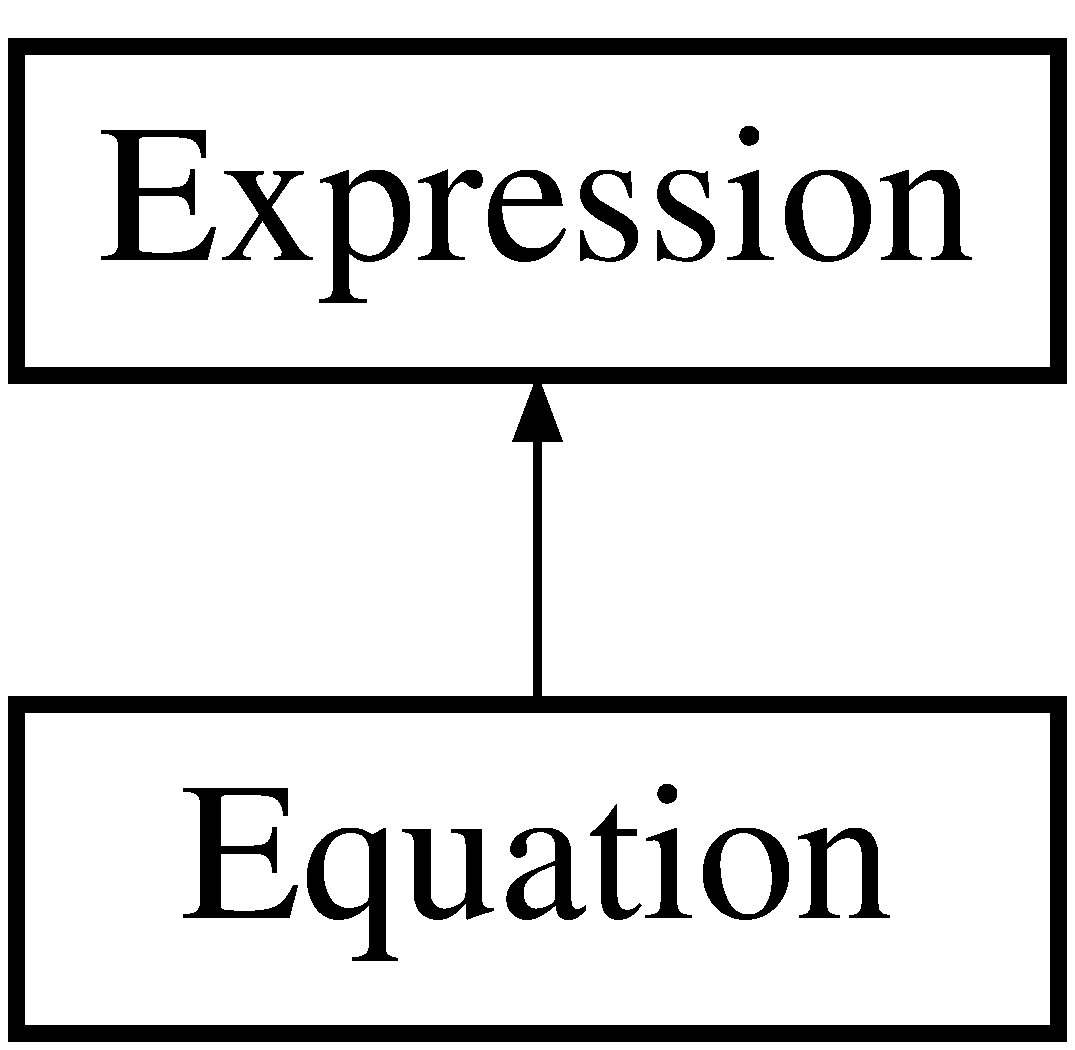
\includegraphics[height=2.000000cm]{class_equation}
\end{center}
\end{figure}
\subsection*{Public Member Functions}
\begin{DoxyCompactItemize}
\item 
\hypertarget{class_equation_aed2c4b2738e9cb3c0746faa098c834e3}{}{\bfseries Equation} (string str\+Eqin, int mode\+Express, int mode\+Equation, int mode\+Number)\label{class_equation_aed2c4b2738e9cb3c0746faa098c834e3}

\item 
\hypertarget{class_equation_a12c17c379993f3ca74d3c9554a977377}{}{\bfseries Equation} (const \hyperlink{class_equation}{Equation} \&)\label{class_equation_a12c17c379993f3ca74d3c9554a977377}

\item 
\hypertarget{class_equation_a868f0c41076b82a30a280100bd7d3402}{}\hyperlink{class_equation}{Equation} \& {\bfseries operator=} (const \hyperlink{class_equation}{Equation} \&)\label{class_equation_a868f0c41076b82a30a280100bd7d3402}

\item 
\hypertarget{class_equation_a2c778077ebd9c7a3f5b5e0889ac58784}{}string {\bfseries Get\+Result} ()\label{class_equation_a2c778077ebd9c7a3f5b5e0889ac58784}

\item 
\hypertarget{class_equation_afbca132bd94e8bcb73e33222a5853397}{}void {\bfseries Solve\+Mathematical} ()\label{class_equation_afbca132bd94e8bcb73e33222a5853397}

\item 
\hypertarget{class_equation_a908a02ec6e453f7cd812f7f9226c138f}{}void {\bfseries Solve\+Logical} ()\label{class_equation_a908a02ec6e453f7cd812f7f9226c138f}

\item 
\hypertarget{class_equation_a4db683603847c120852cfb6ab03388d8}{}\hyperlink{class_number}{Number} $\ast$ {\bfseries Calculate\+Number} (\hyperlink{class_number}{Number} $\ast$opn1, \hyperlink{class_token}{Token} $\ast$opr, \hyperlink{class_number}{Number} $\ast$opn2)\label{class_equation_a4db683603847c120852cfb6ab03388d8}

\item 
\hypertarget{class_equation_aec120c579438bd2a8aa6ab63b87a034e}{}\hyperlink{class_logic}{Logic} $\ast$ {\bfseries Calculate\+Logic} (\hyperlink{class_logic}{Logic} $\ast$opn1, \hyperlink{class_token}{Token} $\ast$opr, \hyperlink{class_logic}{Logic} $\ast$opn2)\label{class_equation_aec120c579438bd2a8aa6ab63b87a034e}

\item 
\hypertarget{class_equation_ad6d9f2b21a528864ab0ef3056895c27c}{}\hyperlink{class_logic}{Logic} $\ast$ {\bfseries Calculate\+Number\+To\+Logic} (\hyperlink{class_number}{Number} $\ast$opn1, \hyperlink{class_token}{Token} $\ast$opr, \hyperlink{class_number}{Number} $\ast$opn2)\label{class_equation_ad6d9f2b21a528864ab0ef3056895c27c}

\end{DoxyCompactItemize}
\subsection*{Additional Inherited Members}


The documentation for this class was generated from the following files\+:\begin{DoxyCompactItemize}
\item 
Equation/Equation.\+h\item 
Equation/Equation.\+cpp\end{DoxyCompactItemize}

\hypertarget{class_equation_exception}{}\section{Equation\+Exception Class Reference}
\label{class_equation_exception}\index{Equation\+Exception@{Equation\+Exception}}
\subsection*{Public Member Functions}
\begin{DoxyCompactItemize}
\item 
\hypertarget{class_equation_exception_a6e4d39e1106b74b1fe9bd3ff1db65572}{}{\bfseries Equation\+Exception} (int)\label{class_equation_exception_a6e4d39e1106b74b1fe9bd3ff1db65572}

\item 
\hypertarget{class_equation_exception_a5d422611e1fdc10ffae5b35fdd6b8a94}{}{\bfseries Equation\+Exception} (const \hyperlink{class_equation_exception}{Equation\+Exception} \&)\label{class_equation_exception_a5d422611e1fdc10ffae5b35fdd6b8a94}

\item 
\hypertarget{class_equation_exception_a7136df9925f88b6c0e85ba9363f632eb}{}const int {\bfseries get\+I\+D} ()\label{class_equation_exception_a7136df9925f88b6c0e85ba9363f632eb}

\item 
\hypertarget{class_equation_exception_ab26d2fcc03011ba4063ee7d24b8ba5bd}{}string {\bfseries get\+Message} ()\label{class_equation_exception_ab26d2fcc03011ba4063ee7d24b8ba5bd}

\end{DoxyCompactItemize}
\subsection*{Static Public Member Functions}
\begin{DoxyCompactItemize}
\item 
\hypertarget{class_equation_exception_ad7639fb8008ee527423d885a78328157}{}static int {\bfseries get\+Num\+Of\+Exception} ()\label{class_equation_exception_ad7639fb8008ee527423d885a78328157}

\end{DoxyCompactItemize}
\subsection*{Static Public Attributes}
\begin{DoxyCompactItemize}
\item 
\hypertarget{class_equation_exception_ae01ec39f2795669551c6e9c780c9befa}{}static const int {\bfseries Out\+Of\+Bound\+Romawi} = 0\label{class_equation_exception_ae01ec39f2795669551c6e9c780c9befa}

\item 
\hypertarget{class_equation_exception_a5c3aa3b5efcb230cb72ab97fa8ba9b57}{}static const int {\bfseries Divide\+By\+Zero} = 1\label{class_equation_exception_a5c3aa3b5efcb230cb72ab97fa8ba9b57}

\item 
\hypertarget{class_equation_exception_aa685b474487c140e4f7b39b328ab8043}{}static const int {\bfseries Modulo\+By\+Non\+Positif} = 2\label{class_equation_exception_aa685b474487c140e4f7b39b328ab8043}

\item 
\hypertarget{class_equation_exception_a31ce87bcca07a6f5495ccb0ad38b03a9}{}static const int {\bfseries Undefined\+Operator} = 3\label{class_equation_exception_a31ce87bcca07a6f5495ccb0ad38b03a9}

\item 
\hypertarget{class_equation_exception_ac0bd8b25068211c372f0bb1939283076}{}static const int {\bfseries Illegal\+Using\+Operator} = 4\label{class_equation_exception_ac0bd8b25068211c372f0bb1939283076}

\item 
\hypertarget{class_equation_exception_a7366915be3f48995b0f43fb22db905d5}{}static const int {\bfseries Empty\+Equation} = 5\label{class_equation_exception_a7366915be3f48995b0f43fb22db905d5}

\end{DoxyCompactItemize}


The documentation for this class was generated from the following files\+:\begin{DoxyCompactItemize}
\item 
Equation\+Exception/Equation\+Exception.\+h\item 
Equation\+Exception/Equation\+Exception.\+cpp\end{DoxyCompactItemize}

\hypertarget{class_expression}{}\section{Expression Class Reference}
\label{class_expression}\index{Expression@{Expression}}
Inheritance diagram for Expression\+:\begin{figure}[H]
\begin{center}
\leavevmode
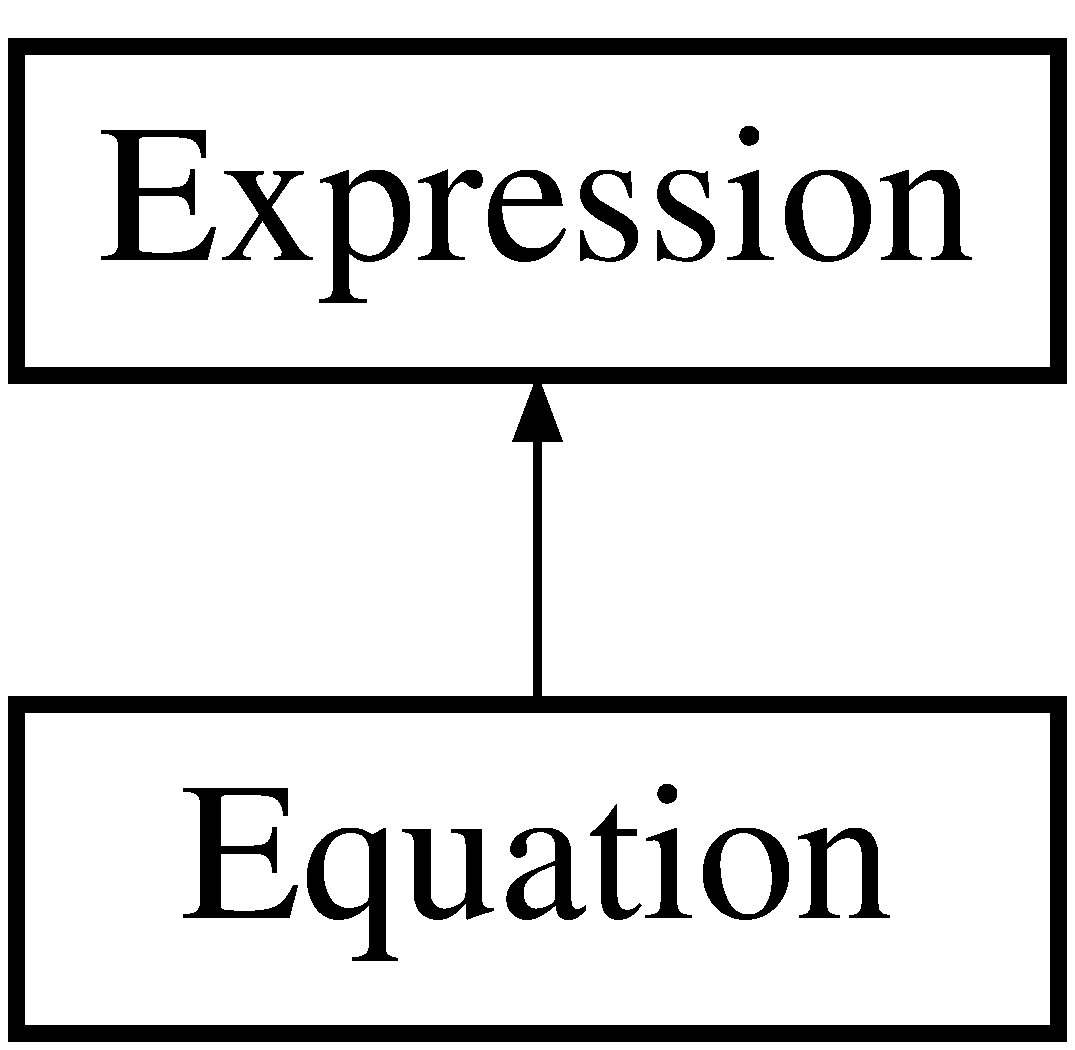
\includegraphics[height=2.000000cm]{class_expression}
\end{center}
\end{figure}
\subsection*{Public Member Functions}
\begin{DoxyCompactItemize}
\item 
\hypertarget{class_expression_a66f8d26da99a31ee208cbcba6f95b71b}{}{\bfseries Expression} (const string \&str\+Exp, int mode\+Expression, int mode\+Equation, int mode\+Number)\label{class_expression_a66f8d26da99a31ee208cbcba6f95b71b}

\item 
\hypertarget{class_expression_a568506b67cd65c7f8c2885c9146c98bd}{}{\bfseries Expression} (const \hyperlink{class_expression}{Expression} \&)\label{class_expression_a568506b67cd65c7f8c2885c9146c98bd}

\end{DoxyCompactItemize}
\subsection*{Protected Attributes}
\begin{DoxyCompactItemize}
\item 
\hypertarget{class_expression_a249c583f1a0ec2aa5e703be12c2e512f}{}\hyperlink{classstack}{stack}$<$ \hyperlink{class_token}{Token} $\ast$ $>$ {\bfseries \+\_\+stack\+Token}\label{class_expression_a249c583f1a0ec2aa5e703be12c2e512f}

\end{DoxyCompactItemize}


The documentation for this class was generated from the following files\+:\begin{DoxyCompactItemize}
\item 
Equation/Expression.\+h\item 
Equation/Expression.\+cpp\end{DoxyCompactItemize}

\hypertarget{class_extension}{}\section{Extension Class Reference}
\label{class_extension}\index{Extension@{Extension}}


Kelas \hyperlink{class_extension}{Extension} berisi konstanta yang dibutuhkan dalam program.  




{\ttfamily \#include $<$Extension.\+h$>$}

\subsection*{Public Member Functions}
\begin{DoxyCompactItemize}
\item 
\hypertarget{class_extension_add927117e09bb09a0d83e3cd3439a15d}{}\hyperlink{class_extension_add927117e09bb09a0d83e3cd3439a15d}{Extension} ()\label{class_extension_add927117e09bb09a0d83e3cd3439a15d}

\begin{DoxyCompactList}\small\item\em Konstruktor kelas \hyperlink{class_extension}{Extension}. \end{DoxyCompactList}\item 
\hypertarget{class_extension_a52c2b4e48fa3f78511b72d55fefcb48c}{}\hyperlink{class_extension_a52c2b4e48fa3f78511b72d55fefcb48c}{$\sim$\+Extension} ()\label{class_extension_a52c2b4e48fa3f78511b72d55fefcb48c}

\begin{DoxyCompactList}\small\item\em Desktruktor kelas \hyperlink{class_extension}{Extension}. \end{DoxyCompactList}\end{DoxyCompactItemize}
\subsection*{Static Public Attributes}
\begin{DoxyCompactItemize}
\item 
\hypertarget{class_extension_a56fbee85e2edb251125b83250c27213c}{}static const int {\bfseries Prefix} = 0\label{class_extension_a56fbee85e2edb251125b83250c27213c}

\item 
\hypertarget{class_extension_a47d3403a109250b3bc0174fdb1de1f71}{}static const int {\bfseries Infix} = 1\label{class_extension_a47d3403a109250b3bc0174fdb1de1f71}

\item 
\hypertarget{class_extension_ad25868fca953adfbd2a22317feaf9b1f}{}static const int {\bfseries Postfix} = 2\label{class_extension_ad25868fca953adfbd2a22317feaf9b1f}

\item 
\hypertarget{class_extension_af88b9749ecfc6e2b25b2a43abc3a5be4}{}static const int {\bfseries Number\+Mode} = 0\label{class_extension_af88b9749ecfc6e2b25b2a43abc3a5be4}

\item 
\hypertarget{class_extension_afa6c3f7ccfba73f7a608424059ee919e}{}static const int {\bfseries Logic\+Mode} = 1\label{class_extension_afa6c3f7ccfba73f7a608424059ee919e}

\item 
\hypertarget{class_extension_aabc020a4a2fe164e7eaebf841ebab7bf}{}static const int {\bfseries Arab\+Mode} = 0\label{class_extension_aabc020a4a2fe164e7eaebf841ebab7bf}

\item 
\hypertarget{class_extension_ac9b5fd4a4e6be30d8d5ffe40342a7d22}{}static const int {\bfseries Romawi\+Mode} = 1\label{class_extension_ac9b5fd4a4e6be30d8d5ffe40342a7d22}

\item 
\hypertarget{class_extension_a60cc91398e9647450ee1211840b816cf}{}static const int {\bfseries default\+Expression\+Mode} = Infix\label{class_extension_a60cc91398e9647450ee1211840b816cf}

\item 
\hypertarget{class_extension_a5ab0b5b49a4ee3276b0b65acaefaf7ac}{}static const int {\bfseries default\+Equation\+Mode} = Number\+Mode\label{class_extension_a5ab0b5b49a4ee3276b0b65acaefaf7ac}

\item 
\hypertarget{class_extension_ac3e873d85dbb68e5524e7f54181f1298}{}static const int {\bfseries default\+Number\+Mode} = Arab\+Mode\label{class_extension_ac3e873d85dbb68e5524e7f54181f1298}

\end{DoxyCompactItemize}


\subsection{Detailed Description}
Kelas \hyperlink{class_extension}{Extension} berisi konstanta yang dibutuhkan dalam program. 

\begin{DoxyAuthor}{Author}
Luqman A. Siswanto (13513024) 
\end{DoxyAuthor}
\begin{DoxyVersion}{Version}
1.\+0
\end{DoxyVersion}
\hypertarget{class_logger_Description}{}\subsection{Description}\label{class_logger_Description}


The documentation for this class was generated from the following files\+:\begin{DoxyCompactItemize}
\item 
Extension/Extension.\+h\item 
Extension/Extension.\+cpp\end{DoxyCompactItemize}

\hypertarget{classlist}{}\section{list$<$ T $>$ Class Template Reference}
\label{classlist}\index{list$<$ T $>$@{list$<$ T $>$}}
\subsection*{Public Member Functions}
\begin{DoxyCompactItemize}
\item 
\hypertarget{classlist_a5f317b0f566c0b9ca0f31e0b927fb7e4}{}{\bfseries list} (T \+\_\+tval)\label{classlist_a5f317b0f566c0b9ca0f31e0b927fb7e4}

\item 
\hypertarget{classlist_a244b5f8b92d576a9a84d3587185d10a9}{}{\bfseries list} (T \+\_\+tval, \hyperlink{classlist}{list}$<$ T $>$ $\ast$\+\_\+tnext)\label{classlist_a244b5f8b92d576a9a84d3587185d10a9}

\item 
\hypertarget{classlist_a2347224ab08486ac9966d598d6ed5743}{}{\bfseries list} (\hyperlink{classlist}{list}$<$ T $>$ \&)\label{classlist_a2347224ab08486ac9966d598d6ed5743}

\item 
\hypertarget{classlist_a6d25919f61226180125992343246c374}{}\hyperlink{classlist}{list}$<$ T $>$ $\ast$ {\bfseries Get\+Next} ()\label{classlist_a6d25919f61226180125992343246c374}

\item 
\hypertarget{classlist_a1e907f5f88c3f4861316c47a5821f31d}{}void {\bfseries Set\+Next} (\hyperlink{classlist}{list}$<$ T $>$ $\ast$\+\_\+tnext)\label{classlist_a1e907f5f88c3f4861316c47a5821f31d}

\item 
\hypertarget{classlist_a8ecb1aeedfd25cda4e506529323a8e8b}{}T \& {\bfseries Get\+Val} ()\label{classlist_a8ecb1aeedfd25cda4e506529323a8e8b}

\item 
\hypertarget{classlist_a83dfea25e06088dc9d0d7cab6317b057}{}void {\bfseries Set\+Val} (T \+\_\+tval)\label{classlist_a83dfea25e06088dc9d0d7cab6317b057}

\end{DoxyCompactItemize}


The documentation for this class was generated from the following file\+:\begin{DoxyCompactItemize}
\item 
Stack/stack.\+h\end{DoxyCompactItemize}

\hypertarget{class_log}{}\section{Log Class Reference}
\label{class_log}\index{Log@{Log}}


Kelas \hyperlink{class_log}{Log} adalah abstract data type untuk log command.  




{\ttfamily \#include $<$Log.\+h$>$}

\subsection*{Public Member Functions}
\begin{DoxyCompactItemize}
\item 
\hypertarget{class_log_af6071a60aa52b6c1b511f99b4bc1b8fe}{}\hyperlink{class_log_af6071a60aa52b6c1b511f99b4bc1b8fe}{Log} ()\label{class_log_af6071a60aa52b6c1b511f99b4bc1b8fe}

\begin{DoxyCompactList}\small\item\em Konstruktor kelas \hyperlink{class_log}{Log}. \end{DoxyCompactList}\item 
\hyperlink{class_log_a0f45072d0b622c4d4f70bb0ef63bef42}{Log} (int, string)
\begin{DoxyCompactList}\small\item\em Konstruktor kelas \hyperlink{class_log}{Log} dengan parameter. \end{DoxyCompactList}\item 
\hyperlink{class_log_a60fc11c5c263c4bfad3f9561a4881a13}{Log} (const \hyperlink{class_log}{Log} \&)
\begin{DoxyCompactList}\small\item\em Copy Constructor kelas \hyperlink{class_log}{Log}. \end{DoxyCompactList}\item 
\hyperlink{class_log}{Log} \& \hyperlink{class_log_a91f9df208ee0515b6403210497d37ee4}{operator=} (const \hyperlink{class_log}{Log} \&)
\begin{DoxyCompactList}\small\item\em Operator assignment kelas \hyperlink{class_log}{Log}. \end{DoxyCompactList}\item 
\hypertarget{class_log_a0fbfda88fbee5027c89f6eb121059360}{}\hyperlink{class_log_a0fbfda88fbee5027c89f6eb121059360}{$\sim$\+Log} ()\label{class_log_a0fbfda88fbee5027c89f6eb121059360}

\begin{DoxyCompactList}\small\item\em Destruktor kelas \hyperlink{class_log}{Log}. \end{DoxyCompactList}\item 
int \hyperlink{class_log_a14536320d9f23ef128cdb004a82d2b83}{Get\+I\+D} ()
\begin{DoxyCompactList}\small\item\em Getter untuk I\+D. \end{DoxyCompactList}\item 
string \hyperlink{class_log_af9f902b597baafe71409025441f0a3e0}{Get\+Sentence} ()
\begin{DoxyCompactList}\small\item\em Getter untuk kalimat log. \end{DoxyCompactList}\item 
void \hyperlink{class_log_a1461ddc76218e915e28d6448c35057ec}{Set\+I\+D} (int)
\begin{DoxyCompactList}\small\item\em Setter untuk I\+D. \end{DoxyCompactList}\item 
void \hyperlink{class_log_a312454df078b83a74e5559f2dd1d69ea}{Set\+Sentence} (string)
\begin{DoxyCompactList}\small\item\em Setter untuk sentence. \end{DoxyCompactList}\end{DoxyCompactItemize}


\subsection{Detailed Description}
Kelas \hyperlink{class_log}{Log} adalah abstract data type untuk log command. 

\begin{DoxyAuthor}{Author}
Luqman A. Siswanto (13513024) 
\end{DoxyAuthor}
\begin{DoxyVersion}{Version}
1.\+0
\end{DoxyVersion}
\hypertarget{class_logger_Description}{}\subsection{Description}\label{class_logger_Description}


\subsection{Constructor \& Destructor Documentation}
\hypertarget{class_log_a0f45072d0b622c4d4f70bb0ef63bef42}{}\index{Log@{Log}!Log@{Log}}
\index{Log@{Log}!Log@{Log}}
\subsubsection[{Log}]{\setlength{\rightskip}{0pt plus 5cm}Log\+::\+Log (
\begin{DoxyParamCaption}
\item[{int}]{id, }
\item[{string}]{sentence}
\end{DoxyParamCaption}
)}\label{class_log_a0f45072d0b622c4d4f70bb0ef63bef42}


Konstruktor kelas \hyperlink{class_log}{Log} dengan parameter. 


\begin{DoxyParams}{Parameters}
{\em int} & -\/ I\+D. \\
\hline
{\em string} & -\/ command pada log yang akan disimpan \\
\hline
\end{DoxyParams}
\hypertarget{class_log_a60fc11c5c263c4bfad3f9561a4881a13}{}\index{Log@{Log}!Log@{Log}}
\index{Log@{Log}!Log@{Log}}
\subsubsection[{Log}]{\setlength{\rightskip}{0pt plus 5cm}Log\+::\+Log (
\begin{DoxyParamCaption}
\item[{const {\bf Log} \&}]{log}
\end{DoxyParamCaption}
)}\label{class_log_a60fc11c5c263c4bfad3f9561a4881a13}


Copy Constructor kelas \hyperlink{class_log}{Log}. 


\begin{DoxyParams}{Parameters}
{\em \hyperlink{class_log}{Log}} & yang akan di-\/copy. \\
\hline
\end{DoxyParams}


\subsection{Member Function Documentation}
\hypertarget{class_log_a14536320d9f23ef128cdb004a82d2b83}{}\index{Log@{Log}!Get\+I\+D@{Get\+I\+D}}
\index{Get\+I\+D@{Get\+I\+D}!Log@{Log}}
\subsubsection[{Get\+I\+D}]{\setlength{\rightskip}{0pt plus 5cm}int Log\+::\+Get\+I\+D (
\begin{DoxyParamCaption}
{}
\end{DoxyParamCaption}
)}\label{class_log_a14536320d9f23ef128cdb004a82d2b83}


Getter untuk I\+D. 

\begin{DoxyReturn}{Returns}
int -\/ I\+D pada log. 
\end{DoxyReturn}
\hypertarget{class_log_af9f902b597baafe71409025441f0a3e0}{}\index{Log@{Log}!Get\+Sentence@{Get\+Sentence}}
\index{Get\+Sentence@{Get\+Sentence}!Log@{Log}}
\subsubsection[{Get\+Sentence}]{\setlength{\rightskip}{0pt plus 5cm}string Log\+::\+Get\+Sentence (
\begin{DoxyParamCaption}
{}
\end{DoxyParamCaption}
)}\label{class_log_af9f902b597baafe71409025441f0a3e0}


Getter untuk kalimat log. 

\begin{DoxyReturn}{Returns}
string -\/ sentence. 
\end{DoxyReturn}
\hypertarget{class_log_a91f9df208ee0515b6403210497d37ee4}{}\index{Log@{Log}!operator=@{operator=}}
\index{operator=@{operator=}!Log@{Log}}
\subsubsection[{operator=}]{\setlength{\rightskip}{0pt plus 5cm}{\bf Log} \& Log\+::operator= (
\begin{DoxyParamCaption}
\item[{const {\bf Log} \&}]{log}
\end{DoxyParamCaption}
)}\label{class_log_a91f9df208ee0515b6403210497d37ee4}


Operator assignment kelas \hyperlink{class_log}{Log}. 


\begin{DoxyParams}{Parameters}
{\em \hyperlink{class_log}{Log}} & yang akan di-\/copy. \\
\hline
\end{DoxyParams}
\hypertarget{class_log_a1461ddc76218e915e28d6448c35057ec}{}\index{Log@{Log}!Set\+I\+D@{Set\+I\+D}}
\index{Set\+I\+D@{Set\+I\+D}!Log@{Log}}
\subsubsection[{Set\+I\+D}]{\setlength{\rightskip}{0pt plus 5cm}void Log\+::\+Set\+I\+D (
\begin{DoxyParamCaption}
\item[{int}]{id}
\end{DoxyParamCaption}
)}\label{class_log_a1461ddc76218e915e28d6448c35057ec}


Setter untuk I\+D. 


\begin{DoxyParams}{Parameters}
{\em int} & -\/ I\+D log. \\
\hline
\end{DoxyParams}
\hypertarget{class_log_a312454df078b83a74e5559f2dd1d69ea}{}\index{Log@{Log}!Set\+Sentence@{Set\+Sentence}}
\index{Set\+Sentence@{Set\+Sentence}!Log@{Log}}
\subsubsection[{Set\+Sentence}]{\setlength{\rightskip}{0pt plus 5cm}void Log\+::\+Set\+Sentence (
\begin{DoxyParamCaption}
\item[{string}]{sentence}
\end{DoxyParamCaption}
)}\label{class_log_a312454df078b83a74e5559f2dd1d69ea}


Setter untuk sentence. 


\begin{DoxyParams}{Parameters}
{\em string} & -\/ sentence. \\
\hline
\end{DoxyParams}


The documentation for this class was generated from the following files\+:\begin{DoxyCompactItemize}
\item 
Logger/Log.\+h\item 
Logger/Log.\+cpp\end{DoxyCompactItemize}

\hypertarget{class_logger}{}\section{Logger Class Reference}
\label{class_logger}\index{Logger@{Logger}}


Kelas \hyperlink{class_log}{Log} adalah abstract data type untuk log command.  




{\ttfamily \#include $<$Logger.\+h$>$}

\subsection*{Public Member Functions}
\begin{DoxyCompactItemize}
\item 
\hypertarget{class_logger_abc41bfb031d896170c7675fa96a6b30c}{}\hyperlink{class_logger_abc41bfb031d896170c7675fa96a6b30c}{Logger} ()\label{class_logger_abc41bfb031d896170c7675fa96a6b30c}

\begin{DoxyCompactList}\small\item\em Konstruktor kelas logger. \end{DoxyCompactList}\item 
\hyperlink{class_logger_a8272fd5aa9d2cfd23c0a785efb84e5aa}{Logger} (\hyperlink{classvector}{vector}$<$ \hyperlink{class_log}{Log} $>$, \hyperlink{classvector}{vector}$<$ \hyperlink{class_log}{Log} $>$)
\begin{DoxyCompactList}\small\item\em Konstruktor kelas logger dengan parameter. \end{DoxyCompactList}\item 
\hyperlink{class_logger_a6d00ba1af86d2af7f048023137df724a}{Logger} (\hyperlink{classvector}{vector}$<$ \hyperlink{class_log}{Log} $>$, \hyperlink{classvector}{vector}$<$ \hyperlink{class_log}{Log} $>$, int)
\begin{DoxyCompactList}\small\item\em Konstruktor kelas logger dengan parameter. \end{DoxyCompactList}\item 
\hyperlink{class_logger_ad1dc4093a3d8c26802357fe2bdb1dabf}{Logger} (const \hyperlink{class_logger}{Logger} \&)
\begin{DoxyCompactList}\small\item\em Copy constructor kelas logger. \end{DoxyCompactList}\item 
\hyperlink{class_logger}{Logger} \& \hyperlink{class_logger_a405b93221b9f3c4293447ed1bf4b77d2}{operator=} (const \hyperlink{class_logger}{Logger} \&)
\begin{DoxyCompactList}\small\item\em Operator assignment kelas \hyperlink{class_logger}{Logger}. \end{DoxyCompactList}\item 
\hypertarget{class_logger_acb668a9e186a25fbaad2e4af6d1ed00a}{}\hyperlink{class_logger_acb668a9e186a25fbaad2e4af6d1ed00a}{$\sim$\+Logger} ()\label{class_logger_acb668a9e186a25fbaad2e4af6d1ed00a}

\begin{DoxyCompactList}\small\item\em Destruktor kelas \hyperlink{class_logger}{Logger}. \end{DoxyCompactList}\item 
\hyperlink{class_log}{Log} \hyperlink{class_logger_a17879024b3d7becb09c6a4f97d3b0864}{Get\+Command} (int)
\begin{DoxyCompactList}\small\item\em Getter \hyperlink{class_log}{Log} Commands dengan indeks tertentu. \end{DoxyCompactList}\item 
\hyperlink{class_log}{Log} \hyperlink{class_logger_a375befae83c2783b4dae46345dab4466}{Get\+Equation} (int)
\begin{DoxyCompactList}\small\item\em Getter \hyperlink{class_log}{Log} Equations dengan indeks tertentu. \end{DoxyCompactList}\item 
int \hyperlink{class_logger_aeabc3b7d9fa5e616649f9779592907dd}{Get\+Size\+Commands} ()
\begin{DoxyCompactList}\small\item\em Getter ukuran commands yang valid. \end{DoxyCompactList}\item 
int \hyperlink{class_logger_a8b8bee01fd0f6e9d1782da3536b57b89}{Get\+Size\+Equations} ()
\begin{DoxyCompactList}\small\item\em Getter ukuran equations yang valid. \end{DoxyCompactList}\item 
\hypertarget{class_logger_a1191038d1044a1121e03cc267e9c681c}{}void \hyperlink{class_logger_a1191038d1044a1121e03cc267e9c681c}{Clear} ()\label{class_logger_a1191038d1044a1121e03cc267e9c681c}

\begin{DoxyCompactList}\small\item\em Menghilangkan seluruh commands dan equations di memori. \end{DoxyCompactList}\item 
\hypertarget{class_logger_a9adae6b89c3f6e6e21fde39fa5028bff}{}void \hyperlink{class_logger_a9adae6b89c3f6e6e21fde39fa5028bff}{Clear\+Commands} ()\label{class_logger_a9adae6b89c3f6e6e21fde39fa5028bff}

\begin{DoxyCompactList}\small\item\em Menghilangkan commands di memori. \end{DoxyCompactList}\item 
\hypertarget{class_logger_a661750c096426b6f5e9d3997720b6850}{}void \hyperlink{class_logger_a661750c096426b6f5e9d3997720b6850}{Clear\+Equations} ()\label{class_logger_a661750c096426b6f5e9d3997720b6850}

\begin{DoxyCompactList}\small\item\em Menghilangkan commands di equations. \end{DoxyCompactList}\item 
void \hyperlink{class_logger_a5b252a46f23b39518ec7984a04b04d5a}{Add\+Command} (\hyperlink{class_log}{Log})
\begin{DoxyCompactList}\small\item\em Menambahkan log pada list of commands. \end{DoxyCompactList}\item 
void \hyperlink{class_logger_a97e6d60cd413fbd1e10f46be2648ffea}{Add\+Equation} (\hyperlink{class_log}{Log})
\begin{DoxyCompactList}\small\item\em Menambahkan log pada list of equations. \end{DoxyCompactList}\item 
int \hyperlink{class_logger_aafe697aae2c001604c9eefde6c858bd7}{Undo\+Equation} (int)
\begin{DoxyCompactList}\small\item\em Membatalkan equation yang telah ditambah. \end{DoxyCompactList}\item 
int \hyperlink{class_logger_ae4db4ef133988b05ebfd290fc882b326}{Redo\+Equation} (int)
\begin{DoxyCompactList}\small\item\em Melakukan kembali equation yang telah di-\/undo. \end{DoxyCompactList}\item 
void \hyperlink{class_logger_a5e42b642372b04412b0489133ccce892}{Show\+Mem} (int)
\begin{DoxyCompactList}\small\item\em Menampilkan memori kembali ke layar. \end{DoxyCompactList}\item 
\hypertarget{class_logger_aa52536c24887d0ba9c9ed52460ef837d}{}void \hyperlink{class_logger_aa52536c24887d0ba9c9ed52460ef837d}{Show\+Mem\+All} ()\label{class_logger_aa52536c24887d0ba9c9ed52460ef837d}

\begin{DoxyCompactList}\small\item\em Menampilkan semua memori kembali ke layar. \end{DoxyCompactList}\end{DoxyCompactItemize}


\subsection{Detailed Description}
Kelas \hyperlink{class_log}{Log} adalah abstract data type untuk log command. 

\begin{DoxyAuthor}{Author}
Luqman A. Siswanto (13513024) 
\end{DoxyAuthor}
\begin{DoxyVersion}{Version}
1.\+0
\end{DoxyVersion}
\hypertarget{class_logger_Description}{}\subsection{Description}\label{class_logger_Description}
\hypertarget{class_logger_Rule}{}\subsection{Rule}\label{class_logger_Rule}
Semua dalam vector commands dijamin valid (tidak ada operasi undo/redo) Seluruh isi vector equations belum tentu valid karena bisa jadi hasil undo 

\subsection{Constructor \& Destructor Documentation}
\hypertarget{class_logger_a8272fd5aa9d2cfd23c0a785efb84e5aa}{}\index{Logger@{Logger}!Logger@{Logger}}
\index{Logger@{Logger}!Logger@{Logger}}
\subsubsection[{Logger}]{\setlength{\rightskip}{0pt plus 5cm}Logger\+::\+Logger (
\begin{DoxyParamCaption}
\item[{{\bf vector}$<$ {\bf Log} $>$}]{commands, }
\item[{{\bf vector}$<$ {\bf Log} $>$}]{equations}
\end{DoxyParamCaption}
)}\label{class_logger_a8272fd5aa9d2cfd23c0a785efb84e5aa}


Konstruktor kelas logger dengan parameter. 


\begin{DoxyParams}{Parameters}
{\em \hyperlink{classvector}{vector$<$\+Log$>$}} & -\/ commands \\
\hline
{\em \hyperlink{classvector}{vector$<$\+Log$>$}} & -\/ equations \\
\hline
\end{DoxyParams}
\hypertarget{class_logger_a6d00ba1af86d2af7f048023137df724a}{}\index{Logger@{Logger}!Logger@{Logger}}
\index{Logger@{Logger}!Logger@{Logger}}
\subsubsection[{Logger}]{\setlength{\rightskip}{0pt plus 5cm}Logger\+::\+Logger (
\begin{DoxyParamCaption}
\item[{{\bf vector}$<$ {\bf Log} $>$}]{commands, }
\item[{{\bf vector}$<$ {\bf Log} $>$}]{equations, }
\item[{int}]{size\+Equations}
\end{DoxyParamCaption}
)}\label{class_logger_a6d00ba1af86d2af7f048023137df724a}


Konstruktor kelas logger dengan parameter. 


\begin{DoxyParams}{Parameters}
{\em \hyperlink{classvector}{vector$<$\+Log$>$}} & -\/ commands \\
\hline
{\em \hyperlink{classvector}{vector$<$\+Log$>$}} & -\/ equations \\
\hline
{\em int} & -\/ ukuran equations yang valid \\
\hline
\end{DoxyParams}
\hypertarget{class_logger_ad1dc4093a3d8c26802357fe2bdb1dabf}{}\index{Logger@{Logger}!Logger@{Logger}}
\index{Logger@{Logger}!Logger@{Logger}}
\subsubsection[{Logger}]{\setlength{\rightskip}{0pt plus 5cm}Logger\+::\+Logger (
\begin{DoxyParamCaption}
\item[{const {\bf Logger} \&}]{logger}
\end{DoxyParamCaption}
)}\label{class_logger_ad1dc4093a3d8c26802357fe2bdb1dabf}


Copy constructor kelas logger. 


\begin{DoxyParams}{Parameters}
{\em \hyperlink{class_logger}{Logger}} & -\/ logger yang akan di-\/copy \\
\hline
\end{DoxyParams}


\subsection{Member Function Documentation}
\hypertarget{class_logger_a5b252a46f23b39518ec7984a04b04d5a}{}\index{Logger@{Logger}!Add\+Command@{Add\+Command}}
\index{Add\+Command@{Add\+Command}!Logger@{Logger}}
\subsubsection[{Add\+Command}]{\setlength{\rightskip}{0pt plus 5cm}void Logger\+::\+Add\+Command (
\begin{DoxyParamCaption}
\item[{{\bf Log}}]{log}
\end{DoxyParamCaption}
)}\label{class_logger_a5b252a46f23b39518ec7984a04b04d5a}


Menambahkan log pada list of commands. 


\begin{DoxyParams}{Parameters}
{\em \hyperlink{class_log}{Log}} & -\/ yang akan ditambah \\
\hline
\end{DoxyParams}
\hypertarget{class_logger_a97e6d60cd413fbd1e10f46be2648ffea}{}\index{Logger@{Logger}!Add\+Equation@{Add\+Equation}}
\index{Add\+Equation@{Add\+Equation}!Logger@{Logger}}
\subsubsection[{Add\+Equation}]{\setlength{\rightskip}{0pt plus 5cm}void Logger\+::\+Add\+Equation (
\begin{DoxyParamCaption}
\item[{{\bf Log}}]{log}
\end{DoxyParamCaption}
)}\label{class_logger_a97e6d60cd413fbd1e10f46be2648ffea}


Menambahkan log pada list of equations. 


\begin{DoxyParams}{Parameters}
{\em \hyperlink{class_log}{Log}} & -\/ yang akan ditambah \\
\hline
\end{DoxyParams}
\hypertarget{class_logger_a17879024b3d7becb09c6a4f97d3b0864}{}\index{Logger@{Logger}!Get\+Command@{Get\+Command}}
\index{Get\+Command@{Get\+Command}!Logger@{Logger}}
\subsubsection[{Get\+Command}]{\setlength{\rightskip}{0pt plus 5cm}{\bf Log} Logger\+::\+Get\+Command (
\begin{DoxyParamCaption}
\item[{int}]{i}
\end{DoxyParamCaption}
)}\label{class_logger_a17879024b3d7becb09c6a4f97d3b0864}


Getter \hyperlink{class_log}{Log} Commands dengan indeks tertentu. 


\begin{DoxyParams}{Parameters}
{\em int} & -\/ indeks \\
\hline
\end{DoxyParams}
\begin{DoxyReturn}{Returns}
\hyperlink{class_log}{Log} -\/ \hyperlink{class_log}{Log} Command dengan indeks tertentu 
\end{DoxyReturn}
\hypertarget{class_logger_a375befae83c2783b4dae46345dab4466}{}\index{Logger@{Logger}!Get\+Equation@{Get\+Equation}}
\index{Get\+Equation@{Get\+Equation}!Logger@{Logger}}
\subsubsection[{Get\+Equation}]{\setlength{\rightskip}{0pt plus 5cm}{\bf Log} Logger\+::\+Get\+Equation (
\begin{DoxyParamCaption}
\item[{int}]{i}
\end{DoxyParamCaption}
)}\label{class_logger_a375befae83c2783b4dae46345dab4466}


Getter \hyperlink{class_log}{Log} Equations dengan indeks tertentu. 


\begin{DoxyParams}{Parameters}
{\em int} & -\/ indeks \\
\hline
\end{DoxyParams}
\begin{DoxyReturn}{Returns}
\hyperlink{class_log}{Log} -\/ \hyperlink{class_log}{Log} \hyperlink{class_equation}{Equation} dengan indeks tertentu 
\end{DoxyReturn}
\hypertarget{class_logger_aeabc3b7d9fa5e616649f9779592907dd}{}\index{Logger@{Logger}!Get\+Size\+Commands@{Get\+Size\+Commands}}
\index{Get\+Size\+Commands@{Get\+Size\+Commands}!Logger@{Logger}}
\subsubsection[{Get\+Size\+Commands}]{\setlength{\rightskip}{0pt plus 5cm}int Logger\+::\+Get\+Size\+Commands (
\begin{DoxyParamCaption}
{}
\end{DoxyParamCaption}
)}\label{class_logger_aeabc3b7d9fa5e616649f9779592907dd}


Getter ukuran commands yang valid. 

\begin{DoxyReturn}{Returns}
int -\/ commands size 
\end{DoxyReturn}
\hypertarget{class_logger_a8b8bee01fd0f6e9d1782da3536b57b89}{}\index{Logger@{Logger}!Get\+Size\+Equations@{Get\+Size\+Equations}}
\index{Get\+Size\+Equations@{Get\+Size\+Equations}!Logger@{Logger}}
\subsubsection[{Get\+Size\+Equations}]{\setlength{\rightskip}{0pt plus 5cm}int Logger\+::\+Get\+Size\+Equations (
\begin{DoxyParamCaption}
{}
\end{DoxyParamCaption}
)}\label{class_logger_a8b8bee01fd0f6e9d1782da3536b57b89}


Getter ukuran equations yang valid. 

\begin{DoxyReturn}{Returns}
int -\/ equations size 
\end{DoxyReturn}
\hypertarget{class_logger_a405b93221b9f3c4293447ed1bf4b77d2}{}\index{Logger@{Logger}!operator=@{operator=}}
\index{operator=@{operator=}!Logger@{Logger}}
\subsubsection[{operator=}]{\setlength{\rightskip}{0pt plus 5cm}{\bf Logger} \& Logger\+::operator= (
\begin{DoxyParamCaption}
\item[{const {\bf Logger} \&}]{logger}
\end{DoxyParamCaption}
)}\label{class_logger_a405b93221b9f3c4293447ed1bf4b77d2}


Operator assignment kelas \hyperlink{class_logger}{Logger}. 


\begin{DoxyParams}{Parameters}
{\em \hyperlink{class_logger}{Logger}} & -\/ logger yang akan di-\/copy \\
\hline
\end{DoxyParams}
\hypertarget{class_logger_ae4db4ef133988b05ebfd290fc882b326}{}\index{Logger@{Logger}!Redo\+Equation@{Redo\+Equation}}
\index{Redo\+Equation@{Redo\+Equation}!Logger@{Logger}}
\subsubsection[{Redo\+Equation}]{\setlength{\rightskip}{0pt plus 5cm}int Logger\+::\+Redo\+Equation (
\begin{DoxyParamCaption}
\item[{int}]{n}
\end{DoxyParamCaption}
)}\label{class_logger_ae4db4ef133988b05ebfd290fc882b326}


Melakukan kembali equation yang telah di-\/undo. 


\begin{DoxyParams}{Parameters}
{\em int} & -\/ berapa item redo yang diminta \\
\hline
\end{DoxyParams}
\begin{DoxyReturn}{Returns}
int -\/ berapa item redo yang berhasil dilakukan 
\end{DoxyReturn}
\hypertarget{class_logger_a5e42b642372b04412b0489133ccce892}{}\index{Logger@{Logger}!Show\+Mem@{Show\+Mem}}
\index{Show\+Mem@{Show\+Mem}!Logger@{Logger}}
\subsubsection[{Show\+Mem}]{\setlength{\rightskip}{0pt plus 5cm}void Logger\+::\+Show\+Mem (
\begin{DoxyParamCaption}
\item[{int}]{n}
\end{DoxyParamCaption}
)}\label{class_logger_a5e42b642372b04412b0489133ccce892}


Menampilkan memori kembali ke layar. 


\begin{DoxyParams}{Parameters}
{\em int} & -\/ berapa item yang akan ditampilkan ke layar \\
\hline
\end{DoxyParams}
\hypertarget{class_logger_aafe697aae2c001604c9eefde6c858bd7}{}\index{Logger@{Logger}!Undo\+Equation@{Undo\+Equation}}
\index{Undo\+Equation@{Undo\+Equation}!Logger@{Logger}}
\subsubsection[{Undo\+Equation}]{\setlength{\rightskip}{0pt plus 5cm}int Logger\+::\+Undo\+Equation (
\begin{DoxyParamCaption}
\item[{int}]{n}
\end{DoxyParamCaption}
)}\label{class_logger_aafe697aae2c001604c9eefde6c858bd7}


Membatalkan equation yang telah ditambah. 


\begin{DoxyParams}{Parameters}
{\em int} & -\/ berapa item undo yang diminta \\
\hline
\end{DoxyParams}
\begin{DoxyReturn}{Returns}
int -\/ berapa item undo yang berhasil dilakukan 
\end{DoxyReturn}


The documentation for this class was generated from the following files\+:\begin{DoxyCompactItemize}
\item 
Logger/Logger.\+h\item 
Logger/Logger.\+cpp\end{DoxyCompactItemize}

\hypertarget{class_logic}{}\section{Logic Class Reference}
\label{class_logic}\index{Logic@{Logic}}
Inheritance diagram for Logic\+:\begin{figure}[H]
\begin{center}
\leavevmode
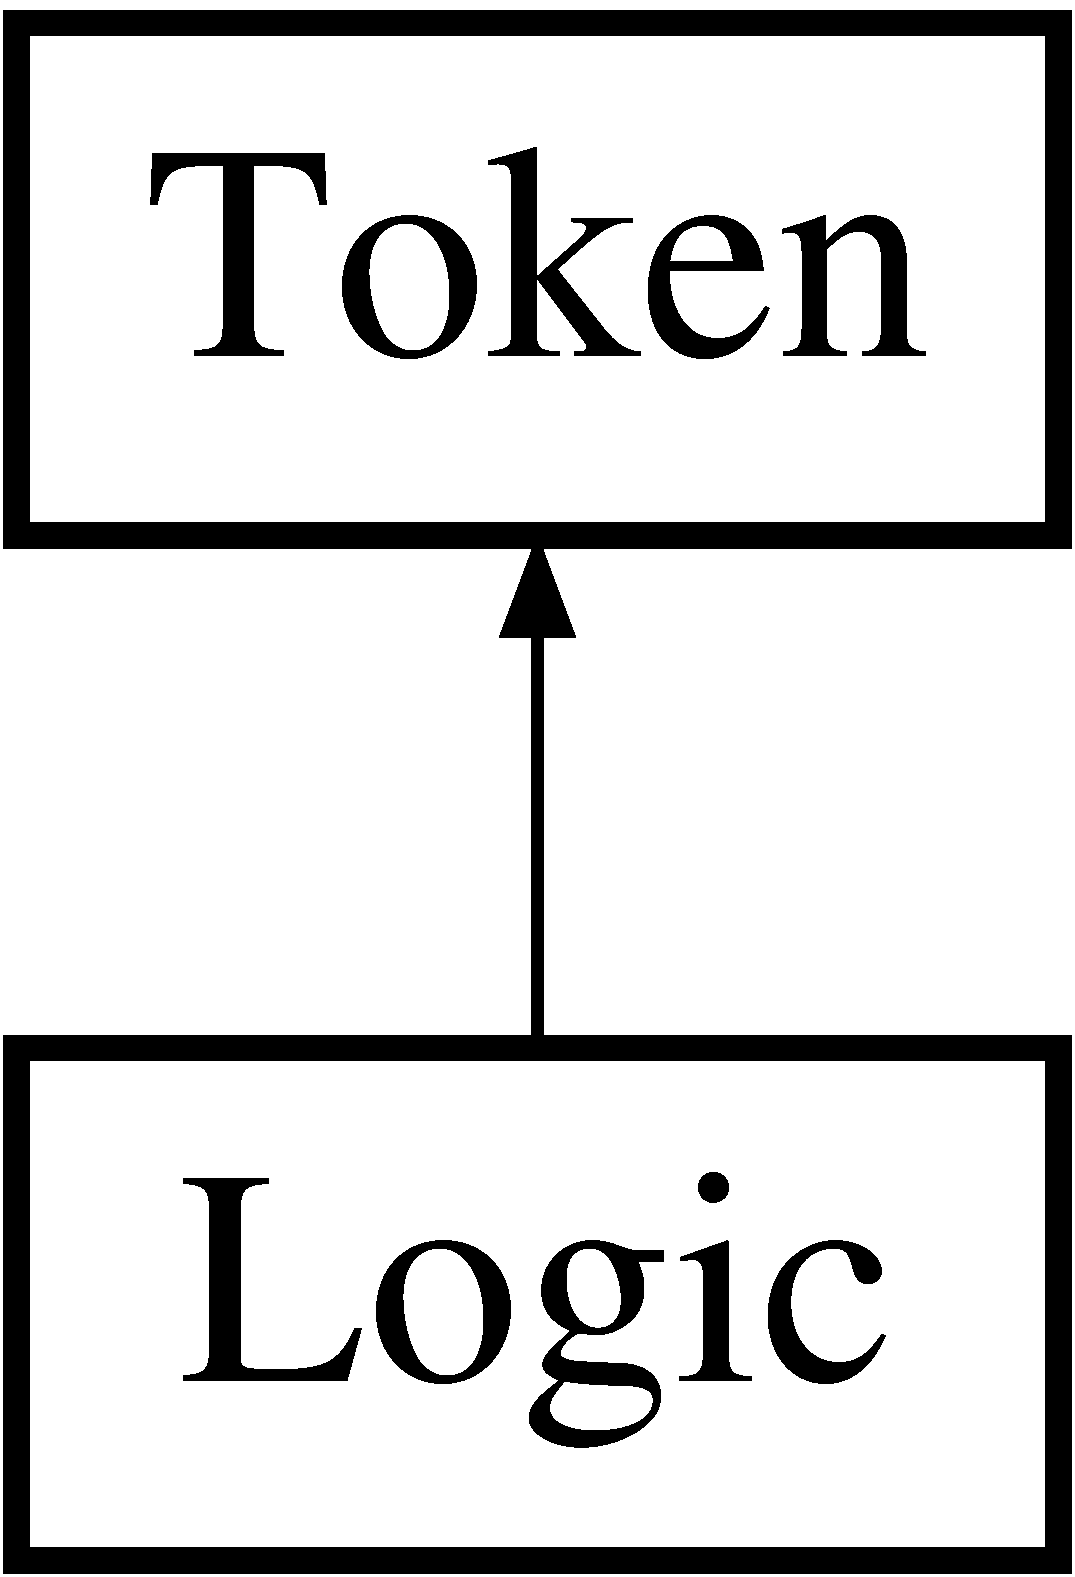
\includegraphics[height=2.000000cm]{class_logic}
\end{center}
\end{figure}
\subsection*{Public Member Functions}
\begin{DoxyCompactItemize}
\item 
\hypertarget{class_logic_a68954cc29f76f2bf6cca7b32adc9552a}{}{\bfseries Logic} (string s)\label{class_logic_a68954cc29f76f2bf6cca7b32adc9552a}

\item 
\hypertarget{class_logic_afdfc186dfdae286243c5cc0fb8c2bfc8}{}{\bfseries Logic} (int i)\label{class_logic_afdfc186dfdae286243c5cc0fb8c2bfc8}

\item 
\hypertarget{class_logic_a038eed90bb481df728efeb289e3ee49d}{}{\bfseries Logic} (const \hyperlink{class_logic}{Logic} \&L)\label{class_logic_a038eed90bb481df728efeb289e3ee49d}

\item 
\hypertarget{class_logic_a8b6abb099b270ff556d660482b1dbc45}{}\hyperlink{class_logic}{Logic} \& {\bfseries operator=} (const \hyperlink{class_logic}{Logic} \&L)\label{class_logic_a8b6abb099b270ff556d660482b1dbc45}

\item 
\hypertarget{class_logic_afd438812fa5e11470f900962ed35a03d}{}int {\bfseries Get\+Logic} ()\label{class_logic_afd438812fa5e11470f900962ed35a03d}

\item 
\hypertarget{class_logic_aa9ce5cce754e20e0a7c0ac9a3ae66629}{}void {\bfseries Set\+Logic} (int i)\label{class_logic_aa9ce5cce754e20e0a7c0ac9a3ae66629}

\item 
\hypertarget{class_logic_a3837982951d720fcbd4c40edfa4d04bf}{}\hyperlink{class_logic}{Logic} \& {\bfseries operator$\sim$} ()\label{class_logic_a3837982951d720fcbd4c40edfa4d04bf}

\item 
\hypertarget{class_logic_a13ed9fa2084d12dbf7194a142d1fbcf6}{}\hyperlink{class_logic}{Logic} \& {\bfseries operator\&} (const \hyperlink{class_logic}{Logic} \&L)\label{class_logic_a13ed9fa2084d12dbf7194a142d1fbcf6}

\item 
\hypertarget{class_logic_a0ee44e200f02d23a34b9f84d42125aa6}{}\hyperlink{class_logic}{Logic} \& {\bfseries operator$\vert$} (const \hyperlink{class_logic}{Logic} \&L)\label{class_logic_a0ee44e200f02d23a34b9f84d42125aa6}

\item 
\hypertarget{class_logic_a80bb6d4a5321494eaaee00f84e4b669b}{}\hyperlink{class_logic}{Logic} \& {\bfseries operator$^\wedge$} (const \hyperlink{class_logic}{Logic} \&L)\label{class_logic_a80bb6d4a5321494eaaee00f84e4b669b}

\item 
\hypertarget{class_logic_a2c4be19b8faf7982cfe5a658d3621c8d}{}int {\bfseries to\+Int} (string)\label{class_logic_a2c4be19b8faf7982cfe5a658d3621c8d}

\item 
\hypertarget{class_logic_adfebd6cf72df68d970e6a404859195b0}{}string {\bfseries to\+String} (int)\label{class_logic_adfebd6cf72df68d970e6a404859195b0}

\end{DoxyCompactItemize}


The documentation for this class was generated from the following files\+:\begin{DoxyCompactItemize}
\item 
Logic/Logic.\+h\item 
Logic/Logic.\+cpp\end{DoxyCompactItemize}

\hypertarget{class_number}{}\section{Number Class Reference}
\label{class_number}\index{Number@{Number}}
Inheritance diagram for Number\+:\begin{figure}[H]
\begin{center}
\leavevmode
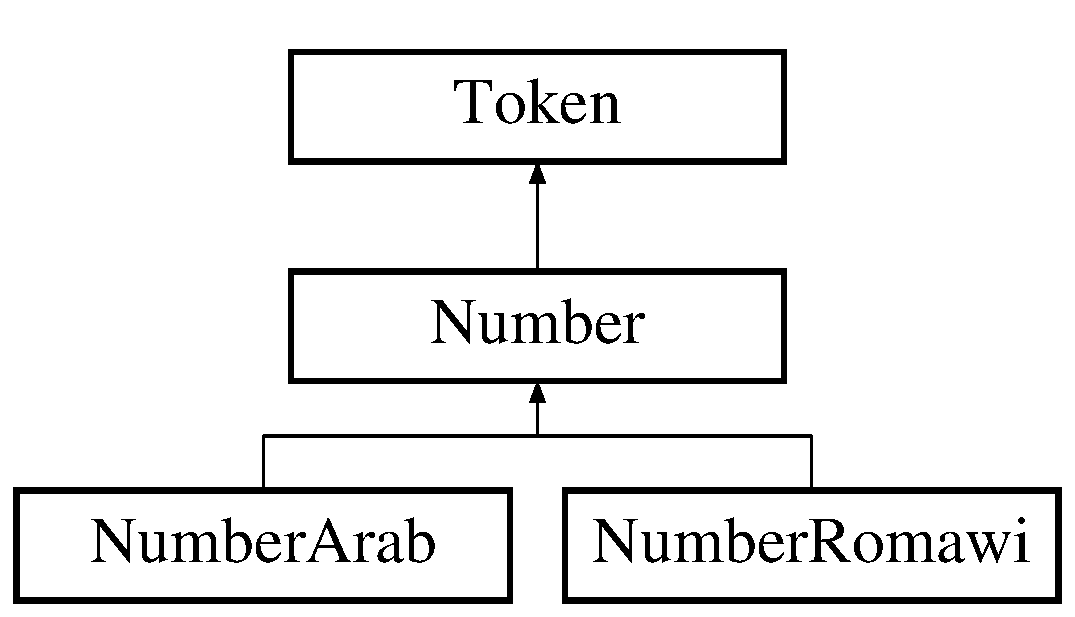
\includegraphics[height=3.000000cm]{class_number}
\end{center}
\end{figure}
\subsection*{Public Member Functions}
\begin{DoxyCompactItemize}
\item 
\hypertarget{class_number_a05d50f9922d3734b4247f6a8764106ee}{}{\bfseries Number} (string s)\label{class_number_a05d50f9922d3734b4247f6a8764106ee}

\item 
\hypertarget{class_number_a7b32779e056a0fcc977d9abf734e852b}{}virtual \hyperlink{class_number}{Number} \& {\bfseries operator=} (\hyperlink{class_number}{Number} \&n)\label{class_number_a7b32779e056a0fcc977d9abf734e852b}

\item 
\hypertarget{class_number_a88ef885d6db4ab0931497cf566ea2055}{}virtual \hyperlink{class_number}{Number} \& {\bfseries operator$\ast$} (const \hyperlink{class_number}{Number} \&)=0\label{class_number_a88ef885d6db4ab0931497cf566ea2055}

\item 
\hypertarget{class_number_abd1476aa7036973a13fa66609794a545}{}virtual \hyperlink{class_number}{Number} \& {\bfseries operator+} (const \hyperlink{class_number}{Number} \&)=0\label{class_number_abd1476aa7036973a13fa66609794a545}

\item 
\hypertarget{class_number_ab2abb500d0885ff5d0acfec32a2b442b}{}virtual \hyperlink{class_number}{Number} \& {\bfseries operator-\/} (const \hyperlink{class_number}{Number} \&)=0\label{class_number_ab2abb500d0885ff5d0acfec32a2b442b}

\item 
\hypertarget{class_number_ad656b7aee20b63427d0cddc57a63d252}{}virtual \hyperlink{class_number}{Number} \& {\bfseries operator/} (const \hyperlink{class_number}{Number} \&)=0\label{class_number_ad656b7aee20b63427d0cddc57a63d252}

\item 
\hypertarget{class_number_a975bf8fc41794c952b02d42165a9ae13}{}virtual \hyperlink{class_number}{Number} \& {\bfseries operator\%} (const \hyperlink{class_number}{Number} \&)=0\label{class_number_a975bf8fc41794c952b02d42165a9ae13}

\item 
\hypertarget{class_number_af5397a992de42b055c126e0dddb0ad9e}{}virtual int {\bfseries to\+Int} (string)=0\label{class_number_af5397a992de42b055c126e0dddb0ad9e}

\item 
\hypertarget{class_number_a27552671ac0f5336e80eb077eabaf6c7}{}virtual string {\bfseries to\+String} (int)=0\label{class_number_a27552671ac0f5336e80eb077eabaf6c7}

\item 
\hypertarget{class_number_a8aae17c6556c5ac901d7e5b586508726}{}\hyperlink{class_logic}{Logic} \& {\bfseries operator$<$} (const \hyperlink{class_number}{Number} \&)\label{class_number_a8aae17c6556c5ac901d7e5b586508726}

\item 
\hypertarget{class_number_a4ab6529135c2b4ddfb6c0dd4c4d0e6e5}{}\hyperlink{class_logic}{Logic} \& {\bfseries operator$<$=} (const \hyperlink{class_number}{Number} \&)\label{class_number_a4ab6529135c2b4ddfb6c0dd4c4d0e6e5}

\item 
\hypertarget{class_number_a75d6669939b25e2a45fa2867db1be330}{}\hyperlink{class_logic}{Logic} \& {\bfseries operator$>$} (const \hyperlink{class_number}{Number} \&)\label{class_number_a75d6669939b25e2a45fa2867db1be330}

\item 
\hypertarget{class_number_aecacb812ffe99815cbac7110bfd82e5f}{}\hyperlink{class_logic}{Logic} \& {\bfseries operator$>$=} (const \hyperlink{class_number}{Number} \&)\label{class_number_aecacb812ffe99815cbac7110bfd82e5f}

\item 
\hypertarget{class_number_ad1a2dc11c69e34d5374a3200b085d8d1}{}\hyperlink{class_logic}{Logic} \& {\bfseries operator==} (const \hyperlink{class_number}{Number} \&)\label{class_number_ad1a2dc11c69e34d5374a3200b085d8d1}

\item 
\hypertarget{class_number_aca8d4626f31071063d33de5466d0c7ec}{}\hyperlink{class_logic}{Logic} \& {\bfseries operator!=} (const \hyperlink{class_number}{Number} \&)\label{class_number_aca8d4626f31071063d33de5466d0c7ec}

\item 
\hypertarget{class_number_a0da0fdbac04873b7320e0730c11f6efe}{}int {\bfseries get\+Nilai} ()\label{class_number_a0da0fdbac04873b7320e0730c11f6efe}

\item 
\hypertarget{class_number_abb7a45c89bf00e7e942f46da59cd5323}{}void {\bfseries set\+Nilai} (int \+\_\+n)\label{class_number_abb7a45c89bf00e7e942f46da59cd5323}

\end{DoxyCompactItemize}
\subsection*{Public Attributes}
\begin{DoxyCompactItemize}
\item 
\hypertarget{class_number_a791a5c270a2b76eb73dbae4aef7fc114}{}int {\bfseries \+\_\+nilai}\label{class_number_a791a5c270a2b76eb73dbae4aef7fc114}

\end{DoxyCompactItemize}


The documentation for this class was generated from the following files\+:\begin{DoxyCompactItemize}
\item 
Number/Number.\+h\item 
Number/Number.\+cpp\end{DoxyCompactItemize}

\hypertarget{class_number_arab}{}\section{Number\+Arab Class Reference}
\label{class_number_arab}\index{Number\+Arab@{Number\+Arab}}
Inheritance diagram for Number\+Arab\+:\begin{figure}[H]
\begin{center}
\leavevmode
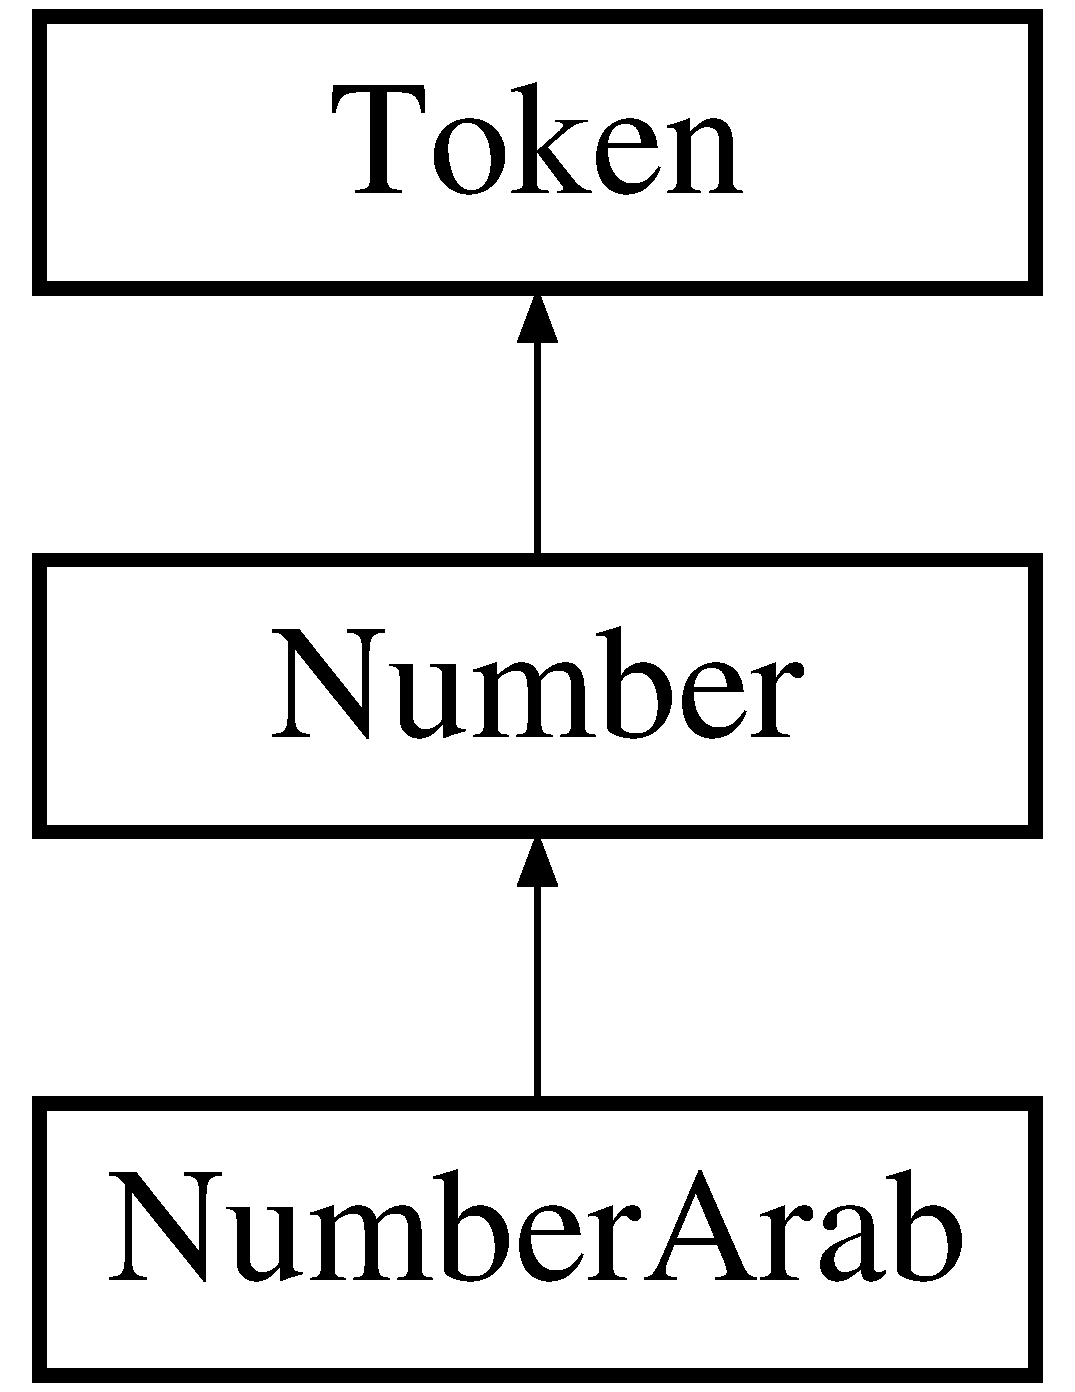
\includegraphics[height=3.000000cm]{class_number_arab}
\end{center}
\end{figure}
\subsection*{Public Member Functions}
\begin{DoxyCompactItemize}
\item 
\hypertarget{class_number_arab_a00678a49c958c39afd33c534f339fd97}{}{\bfseries Number\+Arab} (string s)\label{class_number_arab_a00678a49c958c39afd33c534f339fd97}

\item 
\hypertarget{class_number_arab_a8f82bec543e372dc79497b85ced034f2}{}{\bfseries Number\+Arab} (int \+\_\+n)\label{class_number_arab_a8f82bec543e372dc79497b85ced034f2}

\item 
\hypertarget{class_number_arab_ad109f3f6f71f23afbf0307963f1caece}{}\hyperlink{class_number}{Number} \& {\bfseries operator$\ast$} (const \hyperlink{class_number}{Number} \&)\label{class_number_arab_ad109f3f6f71f23afbf0307963f1caece}

\item 
\hypertarget{class_number_arab_affbc62092236a2be0a3531ed6cffbad4}{}\hyperlink{class_number}{Number} \& {\bfseries operator+} (const \hyperlink{class_number}{Number} \&)\label{class_number_arab_affbc62092236a2be0a3531ed6cffbad4}

\item 
\hypertarget{class_number_arab_aaf42752384e031363284af1fd5eea99d}{}\hyperlink{class_number}{Number} \& {\bfseries operator-\/} (const \hyperlink{class_number}{Number} \&)\label{class_number_arab_aaf42752384e031363284af1fd5eea99d}

\item 
\hypertarget{class_number_arab_a739ba55f7e5528182e3caa9e92a34c65}{}\hyperlink{class_number}{Number} \& {\bfseries operator/} (const \hyperlink{class_number}{Number} \&)\label{class_number_arab_a739ba55f7e5528182e3caa9e92a34c65}

\item 
\hypertarget{class_number_arab_a20016c39977b1d9cce1efe841b472453}{}\hyperlink{class_number}{Number} \& {\bfseries operator\%} (const \hyperlink{class_number}{Number} \&)\label{class_number_arab_a20016c39977b1d9cce1efe841b472453}

\item 
\hypertarget{class_number_arab_af11c9dfb3416eb959d33572fdc96412a}{}int {\bfseries to\+Int} (string s)\label{class_number_arab_af11c9dfb3416eb959d33572fdc96412a}

\item 
\hypertarget{class_number_arab_af8be2e0e0b70595b8405a6078a91e717}{}string {\bfseries to\+String} (int n)\label{class_number_arab_af8be2e0e0b70595b8405a6078a91e717}

\end{DoxyCompactItemize}
\subsection*{Additional Inherited Members}


The documentation for this class was generated from the following files\+:\begin{DoxyCompactItemize}
\item 
Number/Number\+Arab.\+h\item 
Number/Number\+Arab.\+cpp\end{DoxyCompactItemize}

\hypertarget{class_number_romawi}{}\section{Number\+Romawi Class Reference}
\label{class_number_romawi}\index{Number\+Romawi@{Number\+Romawi}}
Inheritance diagram for Number\+Romawi\+:\begin{figure}[H]
\begin{center}
\leavevmode
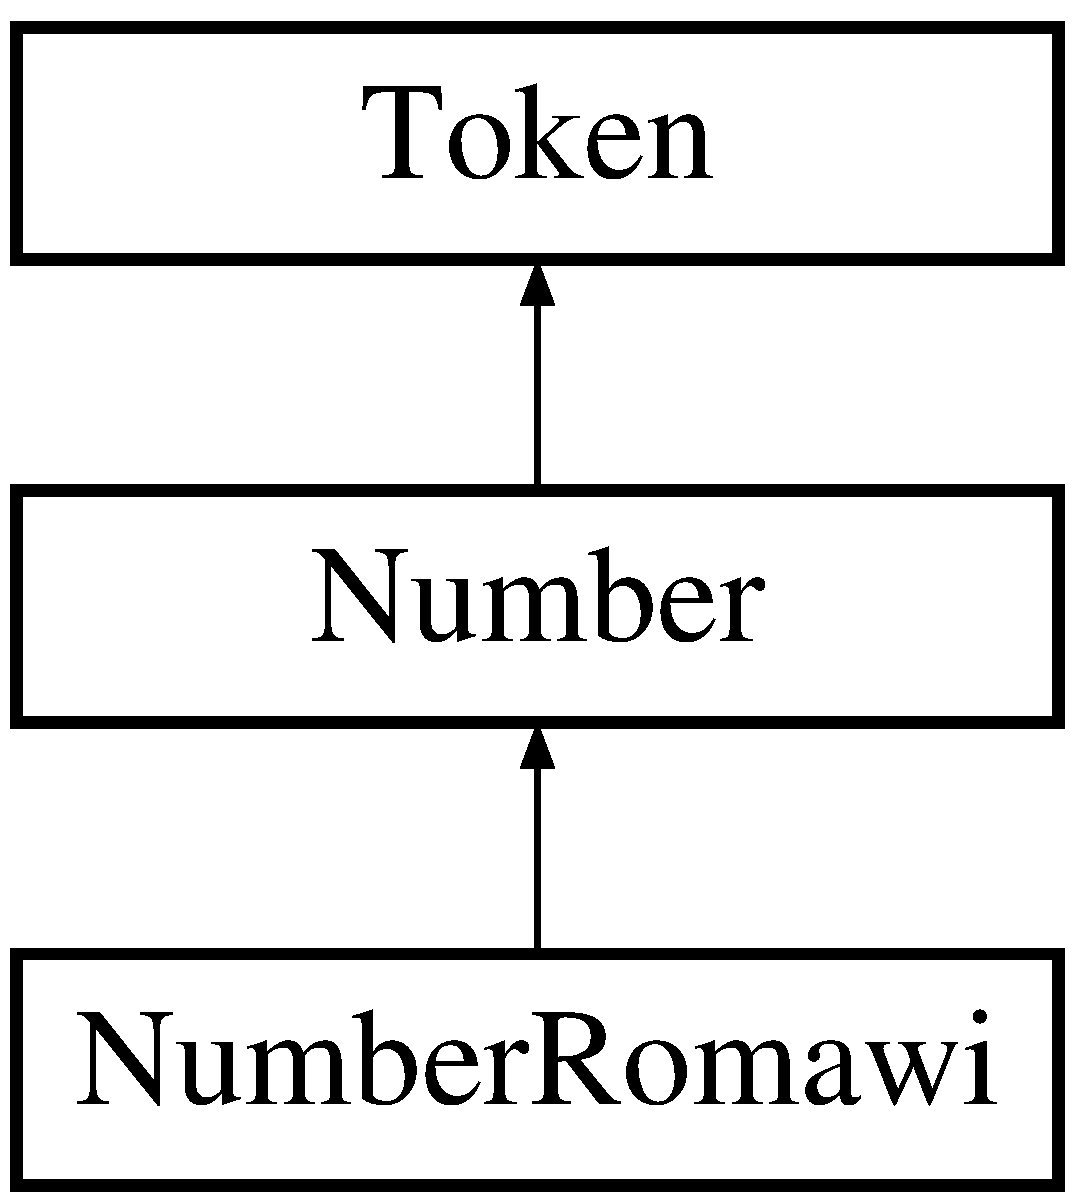
\includegraphics[height=3.000000cm]{class_number_romawi}
\end{center}
\end{figure}
\subsection*{Public Member Functions}
\begin{DoxyCompactItemize}
\item 
\hypertarget{class_number_romawi_a8b059c30a0be899b20764ba0df8ec646}{}{\bfseries Number\+Romawi} (string s)\label{class_number_romawi_a8b059c30a0be899b20764ba0df8ec646}

\item 
\hypertarget{class_number_romawi_ab78eebcc6ff2d7b756d9f039b1a9ffe4}{}{\bfseries Number\+Romawi} (int \+\_\+n)\label{class_number_romawi_ab78eebcc6ff2d7b756d9f039b1a9ffe4}

\item 
\hypertarget{class_number_romawi_acbe2f18994679930c2fb970086a2d675}{}\hyperlink{class_number}{Number} \& {\bfseries operator$\ast$} (const \hyperlink{class_number}{Number} \&)\label{class_number_romawi_acbe2f18994679930c2fb970086a2d675}

\item 
\hypertarget{class_number_romawi_a62aa9142a55197d57516d8fecd995de2}{}\hyperlink{class_number}{Number} \& {\bfseries operator+} (const \hyperlink{class_number}{Number} \&)\label{class_number_romawi_a62aa9142a55197d57516d8fecd995de2}

\item 
\hypertarget{class_number_romawi_a685da03107430d6a63c02f99ce7b39d0}{}\hyperlink{class_number}{Number} \& {\bfseries operator-\/} (const \hyperlink{class_number}{Number} \&)\label{class_number_romawi_a685da03107430d6a63c02f99ce7b39d0}

\item 
\hypertarget{class_number_romawi_a33d1f44531ddb86bb77e0e14b261b3c4}{}\hyperlink{class_number}{Number} \& {\bfseries operator/} (const \hyperlink{class_number}{Number} \&)\label{class_number_romawi_a33d1f44531ddb86bb77e0e14b261b3c4}

\item 
\hypertarget{class_number_romawi_ab1655c4b36a90ceb23a9d33cc63b9f96}{}\hyperlink{class_number}{Number} \& {\bfseries operator\%} (const \hyperlink{class_number}{Number} \&)\label{class_number_romawi_ab1655c4b36a90ceb23a9d33cc63b9f96}

\item 
\hypertarget{class_number_romawi_a7198e8586508321b6a8da6c5ef92cf18}{}int {\bfseries to\+Int} (string s)\label{class_number_romawi_a7198e8586508321b6a8da6c5ef92cf18}

\item 
\hypertarget{class_number_romawi_a5d22c55f63cfb4e1cc7b7f711f91fba7}{}string {\bfseries to\+String} (int n)\label{class_number_romawi_a5d22c55f63cfb4e1cc7b7f711f91fba7}

\end{DoxyCompactItemize}
\subsection*{Additional Inherited Members}


The documentation for this class was generated from the following files\+:\begin{DoxyCompactItemize}
\item 
Number/Number\+Romawi.\+h\item 
Number/Number\+Romawi.\+cpp\end{DoxyCompactItemize}

\hypertarget{class_reader}{}\section{Reader Class Reference}
\label{class_reader}\index{Reader@{Reader}}


Kelas \hyperlink{class_reader}{Reader} bertugas menerima input dari user kemudian mengkategorikan input tersebut termasuk command atau ekspresi.  




{\ttfamily \#include $<$Reader.\+h$>$}

\subsection*{Public Member Functions}
\begin{DoxyCompactItemize}
\item 
\hypertarget{class_reader_adcda31b507720ab44044d7a21686fba2}{}\hyperlink{class_reader_adcda31b507720ab44044d7a21686fba2}{Reader} ()\label{class_reader_adcda31b507720ab44044d7a21686fba2}

\begin{DoxyCompactList}\small\item\em Konstruktor kelas \hyperlink{class_reader}{Reader}. \end{DoxyCompactList}\item 
\hyperlink{class_reader_a22be4123536f4d9a5432290fabb8971c}{Reader} (const \hyperlink{class_reader}{Reader} \&)
\begin{DoxyCompactList}\small\item\em Copy constructor kelas logger. \end{DoxyCompactList}\item 
\hyperlink{class_reader}{Reader} \& \hyperlink{class_reader_ace806a7f7b055341c10af595fedcd5f4}{operator=} (const \hyperlink{class_reader}{Reader} \&)
\begin{DoxyCompactList}\small\item\em Copy constructor kelas logger. \end{DoxyCompactList}\item 
\hypertarget{class_reader_a78089542fd27a0ac2df6702fffe8725c}{}\hyperlink{class_reader_a78089542fd27a0ac2df6702fffe8725c}{$\sim$\+Reader} ()\label{class_reader_a78089542fd27a0ac2df6702fffe8725c}

\begin{DoxyCompactList}\small\item\em Destruktor kelas logger. \end{DoxyCompactList}\item 
string \hyperlink{class_reader_a418c58459e774307fce1d5cc93e23d37}{Read} ()
\begin{DoxyCompactList}\small\item\em Membaca perintah dari user sekaligus meng-\/update data member is\+Equation. \end{DoxyCompactList}\item 
bool \hyperlink{class_reader_aa5bd7ae7e8c0e982124fac3289277990}{Is\+Equation} ()
\begin{DoxyCompactList}\small\item\em Mengembalikan predikat apakah sebuah string merupakan equation. \end{DoxyCompactList}\end{DoxyCompactItemize}


\subsection{Detailed Description}
Kelas \hyperlink{class_reader}{Reader} bertugas menerima input dari user kemudian mengkategorikan input tersebut termasuk command atau ekspresi. 

\begin{DoxyAuthor}{Author}
Luqman A. Siswanto (13513024) 
\end{DoxyAuthor}
\begin{DoxyVersion}{Version}
1.\+0
\end{DoxyVersion}
\hypertarget{class_logger_Description}{}\subsection{Description}\label{class_logger_Description}


\subsection{Constructor \& Destructor Documentation}
\hypertarget{class_reader_a22be4123536f4d9a5432290fabb8971c}{}\index{Reader@{Reader}!Reader@{Reader}}
\index{Reader@{Reader}!Reader@{Reader}}
\subsubsection[{Reader}]{\setlength{\rightskip}{0pt plus 5cm}Reader\+::\+Reader (
\begin{DoxyParamCaption}
\item[{const {\bf Reader} \&}]{r}
\end{DoxyParamCaption}
)}\label{class_reader_a22be4123536f4d9a5432290fabb8971c}


Copy constructor kelas logger. 


\begin{DoxyParams}{Parameters}
{\em \hyperlink{class_reader}{Reader}} & \+: yang akan di-\/copy \\
\hline
\end{DoxyParams}


\subsection{Member Function Documentation}
\hypertarget{class_reader_aa5bd7ae7e8c0e982124fac3289277990}{}\index{Reader@{Reader}!Is\+Equation@{Is\+Equation}}
\index{Is\+Equation@{Is\+Equation}!Reader@{Reader}}
\subsubsection[{Is\+Equation}]{\setlength{\rightskip}{0pt plus 5cm}bool Reader\+::\+Is\+Equation (
\begin{DoxyParamCaption}
{}
\end{DoxyParamCaption}
)}\label{class_reader_aa5bd7ae7e8c0e982124fac3289277990}


Mengembalikan predikat apakah sebuah string merupakan equation. 

\begin{DoxyReturn}{Returns}
bool -\/ jika true, maka string adalah equation 
\end{DoxyReturn}
\hypertarget{class_reader_ace806a7f7b055341c10af595fedcd5f4}{}\index{Reader@{Reader}!operator=@{operator=}}
\index{operator=@{operator=}!Reader@{Reader}}
\subsubsection[{operator=}]{\setlength{\rightskip}{0pt plus 5cm}{\bf Reader} \& Reader\+::operator= (
\begin{DoxyParamCaption}
\item[{const {\bf Reader} \&}]{r}
\end{DoxyParamCaption}
)}\label{class_reader_ace806a7f7b055341c10af595fedcd5f4}


Copy constructor kelas logger. 


\begin{DoxyParams}{Parameters}
{\em \hyperlink{class_reader}{Reader}} & \+: yang akan di-\/copy \\
\hline
\end{DoxyParams}
\hypertarget{class_reader_a418c58459e774307fce1d5cc93e23d37}{}\index{Reader@{Reader}!Read@{Read}}
\index{Read@{Read}!Reader@{Reader}}
\subsubsection[{Read}]{\setlength{\rightskip}{0pt plus 5cm}string Reader\+::\+Read (
\begin{DoxyParamCaption}
{}
\end{DoxyParamCaption}
)}\label{class_reader_a418c58459e774307fce1d5cc93e23d37}


Membaca perintah dari user sekaligus meng-\/update data member is\+Equation. 

\begin{DoxyReturn}{Returns}
string -\/ string yang berhasil dibaca 
\end{DoxyReturn}


The documentation for this class was generated from the following files\+:\begin{DoxyCompactItemize}
\item 
Reader/Reader.\+h\item 
Reader/Reader.\+cpp\end{DoxyCompactItemize}

\hypertarget{class_saver}{}\section{Saver Class Reference}
\label{class_saver}\index{Saver@{Saver}}


Kelas \hyperlink{class_class_controller}{Class\+Controller} bertugas untuk mengatur kehidupan dan kematian kelas-\/kelas lain.  




{\ttfamily \#include $<$Class\+Controller.\+h$>$}

\subsection*{Public Member Functions}
\begin{DoxyCompactItemize}
\item 
\hypertarget{class_saver_a7212120d1c632eeb4086f2d2459d3d85}{}{\bfseries Saver} (string S, \hyperlink{class_logger}{Logger} L)\label{class_saver_a7212120d1c632eeb4086f2d2459d3d85}

\item 
\hypertarget{class_saver_a9bebb09eceb5b95bf4515a6cb9cc7f71}{}string {\bfseries Get\+File\+Name} ()\label{class_saver_a9bebb09eceb5b95bf4515a6cb9cc7f71}

\item 
\hypertarget{class_saver_a056da2a95f516e5cf9601aa78929758b}{}\hyperlink{class_logger}{Logger} {\bfseries Get\+Log\+Memory} ()\label{class_saver_a056da2a95f516e5cf9601aa78929758b}

\item 
\hypertarget{class_saver_a0b712d7e487acee98c0bdaebea59d546}{}void {\bfseries Set\+File\+Name} (string)\label{class_saver_a0b712d7e487acee98c0bdaebea59d546}

\item 
\hypertarget{class_saver_ad7cc8e090549e00fd739a84861c241fb}{}void {\bfseries Set\+Log\+Memory} (\hyperlink{class_logger}{Logger})\label{class_saver_ad7cc8e090549e00fd739a84861c241fb}

\item 
\hypertarget{class_saver_aabeb74d91699a078e367ec2f7903792b}{}void {\bfseries Convert\+To\+File} ()\label{class_saver_aabeb74d91699a078e367ec2f7903792b}

\end{DoxyCompactItemize}


\subsection{Detailed Description}
Kelas \hyperlink{class_class_controller}{Class\+Controller} bertugas untuk mengatur kehidupan dan kematian kelas-\/kelas lain. 

\begin{DoxyAuthor}{Author}
Luqman A. Siswanto (13513024) 
\end{DoxyAuthor}
\begin{DoxyVersion}{Version}
1.\+0
\end{DoxyVersion}
\hypertarget{class_logger_Description}{}\subsection{Description}\label{class_logger_Description}


The documentation for this class was generated from the following files\+:\begin{DoxyCompactItemize}
\item 
Saver/Saver.\+h\item 
Saver/Saver.\+cpp\end{DoxyCompactItemize}

\hypertarget{classstack}{}\section{stack$<$ T $>$ Class Template Reference}
\label{classstack}\index{stack$<$ T $>$@{stack$<$ T $>$}}
\subsection*{Public Member Functions}
\begin{DoxyCompactItemize}
\item 
\hypertarget{classstack_a2ac4beee237e53625290c15afd3a636a}{}{\bfseries stack} (const \hyperlink{classstack}{stack}$<$ T $>$ \&)\label{classstack_a2ac4beee237e53625290c15afd3a636a}

\item 
\hypertarget{classstack_ad4085b42329de4eb6fb1128d21b89359}{}\hyperlink{classstack}{stack}$<$ T $>$ \& {\bfseries operator=} (const \hyperlink{classstack}{stack}$<$ T $>$ \&)\label{classstack_ad4085b42329de4eb6fb1128d21b89359}

\item 
\hypertarget{classstack_ab82d4f94c3a83318499848de576feede}{}bool {\bfseries empty} ()\label{classstack_ab82d4f94c3a83318499848de576feede}

\item 
\hypertarget{classstack_a1577ac10f88c5d6bdbbd9f8f61344b91}{}int {\bfseries size} ()\label{classstack_a1577ac10f88c5d6bdbbd9f8f61344b91}

\item 
\hypertarget{classstack_a12b99509d933115ac110c2fbfea56e5c}{}T \& {\bfseries top} ()\label{classstack_a12b99509d933115ac110c2fbfea56e5c}

\item 
\hypertarget{classstack_a3920cecbc350ae7db943688b8c634719}{}void {\bfseries push} (const T \&)\label{classstack_a3920cecbc350ae7db943688b8c634719}

\item 
\hypertarget{classstack_ad6615a82d944ce2e9a9c260b1d126666}{}void {\bfseries pop} ()\label{classstack_ad6615a82d944ce2e9a9c260b1d126666}

\end{DoxyCompactItemize}


The documentation for this class was generated from the following file\+:\begin{DoxyCompactItemize}
\item 
Stack/stack.\+h\end{DoxyCompactItemize}

\hypertarget{class_token}{}\section{Token Class Reference}
\label{class_token}\index{Token@{Token}}
Inheritance diagram for Token\+:\begin{figure}[H]
\begin{center}
\leavevmode
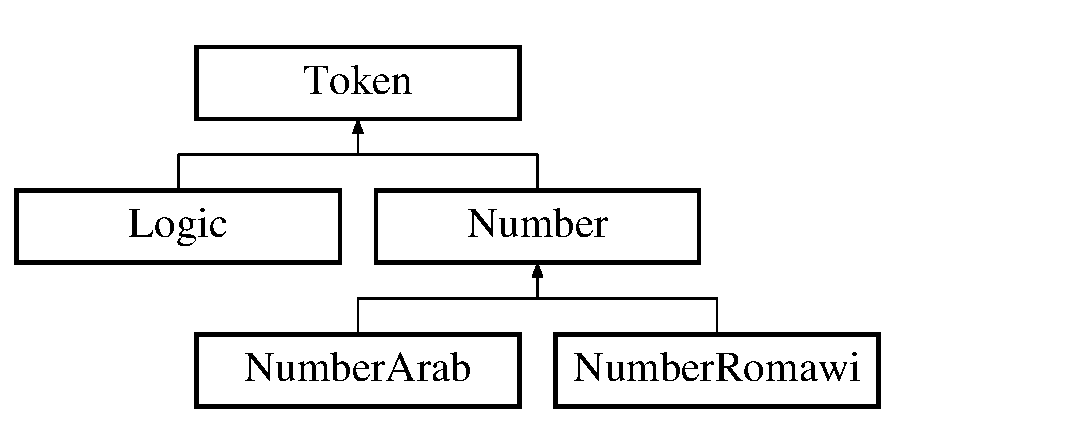
\includegraphics[height=3.000000cm]{class_token}
\end{center}
\end{figure}
\subsection*{Public Member Functions}
\begin{DoxyCompactItemize}
\item 
\hypertarget{class_token_a8e24c1543e23f1ace3483af6528878c1}{}{\bfseries Token} (string S)\label{class_token_a8e24c1543e23f1ace3483af6528878c1}

\item 
\hypertarget{class_token_a68f6e732c2ddfabe4a2cd18630c2b262}{}{\bfseries Token} (const \hyperlink{class_token}{Token} \&T)\label{class_token_a68f6e732c2ddfabe4a2cd18630c2b262}

\item 
\hypertarget{class_token_a6cda5d9c6fad121dc0e4701296c2c507}{}\hyperlink{class_token}{Token} \& {\bfseries operator=} (const \hyperlink{class_token}{Token} \&T)\label{class_token_a6cda5d9c6fad121dc0e4701296c2c507}

\item 
\hypertarget{class_token_a6f7a4603b5915a72ed8b1bdfaf37f05e}{}string {\bfseries Get\+Sym\+Token} () const \label{class_token_a6f7a4603b5915a72ed8b1bdfaf37f05e}

\item 
\hypertarget{class_token_abbd1e32847716e3d2542de00d5a6b96d}{}bool {\bfseries Get\+Is\+Operator} ()\label{class_token_abbd1e32847716e3d2542de00d5a6b96d}

\item 
\hypertarget{class_token_a18edd2d93a149d142b5de2033b40e00b}{}void {\bfseries Set\+Sym\+Token} (string S)\label{class_token_a18edd2d93a149d142b5de2033b40e00b}

\item 
\hypertarget{class_token_a27104e684c8d247ce8b547990fe33f9b}{}int {\bfseries Get\+Prior} ()\label{class_token_a27104e684c8d247ce8b547990fe33f9b}

\end{DoxyCompactItemize}


The documentation for this class was generated from the following files\+:\begin{DoxyCompactItemize}
\item 
Token/Token.\+h\item 
Token/Token.\+cpp\end{DoxyCompactItemize}

\hypertarget{classvector}{}\section{vector$<$ T $>$ Class Template Reference}
\label{classvector}\index{vector$<$ T $>$@{vector$<$ T $>$}}


Vector adalah implementasi vector yang ekuivalen vector S\+T\+L C++.  




{\ttfamily \#include $<$vector.\+h$>$}

\subsection*{Public Member Functions}
\begin{DoxyCompactItemize}
\item 
\hypertarget{classvector_a00d237f22fd5eb1aa9a536993e82e54f}{}\hyperlink{classvector_a00d237f22fd5eb1aa9a536993e82e54f}{vector} ()\label{classvector_a00d237f22fd5eb1aa9a536993e82e54f}

\begin{DoxyCompactList}\small\item\em Konstruktor kelas vector. \end{DoxyCompactList}\item 
\hyperlink{classvector_a14efcceb0fa770e5cd88998d23d49767}{vector} (const \hyperlink{classvector}{vector}$<$ T $>$ \&)
\begin{DoxyCompactList}\small\item\em Copy constructor kelas vector. \end{DoxyCompactList}\item 
\hyperlink{classvector}{vector}$<$ T $>$ \& \hyperlink{classvector_ace0bae2999250693936d58b2530c323b}{operator=} (\hyperlink{classvector}{vector}$<$ T $>$)
\begin{DoxyCompactList}\small\item\em Operator assignment kelas vector. \end{DoxyCompactList}\item 
\hyperlink{classvector_a7bc236f547bb5debe890fa8ebaabe965}{$\sim$vector} ()
\begin{DoxyCompactList}\small\item\em Operator assignment kelas vector. \end{DoxyCompactList}\item 
int \hyperlink{classvector_a00d86ff0224b867efa96488fdfe3a163}{size} ()
\begin{DoxyCompactList}\small\item\em Mengembalikan ukuran vector. \end{DoxyCompactList}\item 
int \hyperlink{classvector_a18af0dd0fba070c03f0c92137016ea90}{max\+\_\+size} ()
\begin{DoxyCompactList}\small\item\em Mengembalikan ukuran maksimal vector saat ini sebelum alokasi kembali. \end{DoxyCompactList}\item 
void \hyperlink{classvector_ad216209d5c4f4c9df7e026eb539e1773}{resize} (int)
\begin{DoxyCompactList}\small\item\em Mengubah ukuran vector. \end{DoxyCompactList}\item 
int \hyperlink{classvector_a00c3fb56dd523269e333428be4b78b9c}{capacity} ()
\begin{DoxyCompactList}\small\item\em Mengembalikan ukuran maksimal vector saat ini sebelum alokasi kembali. \end{DoxyCompactList}\item 
bool \hyperlink{classvector_af342adf8e0f862f5d91b119dd108bf25}{empty} ()
\begin{DoxyCompactList}\small\item\em Mengembalikan predikat apakah vector kosong. \end{DoxyCompactList}\item 
T \& \hyperlink{classvector_a87628125f574ff26aa35e8c7eb726108}{operator\mbox{[}$\,$\mbox{]}} (int)
\begin{DoxyCompactList}\small\item\em Mengembalikan isi kontainer pada indeks tertentu. \end{DoxyCompactList}\item 
T \& \hyperlink{classvector_acb130730b5e99b862bb6770b9c33a6ac}{at} (int)
\begin{DoxyCompactList}\small\item\em Mengembalikan isi kontainer pada indeks tertentu. \end{DoxyCompactList}\item 
T \& \hyperlink{classvector_a60c0c3c2925224f41b2d8405bd138ebb}{front} ()
\begin{DoxyCompactList}\small\item\em Mengembalikan isi kontainer paling awal. \end{DoxyCompactList}\item 
T \& \hyperlink{classvector_a13d864f69391af4f471d111d68c19b9c}{back} ()
\begin{DoxyCompactList}\small\item\em Mengembalikan isi kontainer paling akhir. \end{DoxyCompactList}\item 
void \hyperlink{classvector_a44266e46c0784ef64b478ad9e931ee2e}{push\+\_\+back} (T)
\begin{DoxyCompactList}\small\item\em Memasukkan item pada akhir kontainer. \end{DoxyCompactList}\item 
void \hyperlink{classvector_aeec9e5d602d555d466a936310aa47866}{pop\+\_\+back} ()
\begin{DoxyCompactList}\small\item\em Melepaskan item paling belakang vector. \end{DoxyCompactList}\item 
void \hyperlink{classvector_acb86c331d5493acd8da68386292d5642}{swap} (\hyperlink{classvector}{vector}$<$ T $>$ \&)
\begin{DoxyCompactList}\small\item\em Menukar kontainer vector beserta atributnya dengan vector lain. \end{DoxyCompactList}\item 
\hypertarget{classvector_a1a91cd18e54c382af1097d630405398f}{}void \hyperlink{classvector_a1a91cd18e54c382af1097d630405398f}{clear} ()\label{classvector_a1a91cd18e54c382af1097d630405398f}

\begin{DoxyCompactList}\small\item\em Mengkosongkan isi vector. \end{DoxyCompactList}\end{DoxyCompactItemize}


\subsection{Detailed Description}
\subsubsection*{template$<$class T$>$class vector$<$ T $>$}

Vector adalah implementasi vector yang ekuivalen vector S\+T\+L C++. 

\begin{DoxyAuthor}{Author}
Luqman A. Siswanto (13513024) 
\end{DoxyAuthor}
\begin{DoxyVersion}{Version}
1.\+0
\end{DoxyVersion}
\hypertarget{class_logger_Description}{}\subsection{Description}\label{class_logger_Description}


\subsection{Constructor \& Destructor Documentation}
\hypertarget{classvector_a14efcceb0fa770e5cd88998d23d49767}{}\index{vector@{vector}!vector@{vector}}
\index{vector@{vector}!vector@{vector}}
\subsubsection[{vector}]{\setlength{\rightskip}{0pt plus 5cm}template$<$class T$>$ {\bf vector}$<$ T $>$\+::{\bf vector} (
\begin{DoxyParamCaption}
\item[{const {\bf vector}$<$ T $>$ \&}]{v}
\end{DoxyParamCaption}
)}\label{classvector_a14efcceb0fa770e5cd88998d23d49767}


Copy constructor kelas vector. 


\begin{DoxyParams}{Parameters}
{\em vector} & \+: yang akan di-\/copy \\
\hline
\end{DoxyParams}
\hypertarget{classvector_a7bc236f547bb5debe890fa8ebaabe965}{}\index{vector@{vector}!````~vector@{$\sim$vector}}
\index{````~vector@{$\sim$vector}!vector@{vector}}
\subsubsection[{$\sim$vector}]{\setlength{\rightskip}{0pt plus 5cm}template$<$class T $>$ {\bf vector}$<$ T $>$\+::$\sim${\bf vector} (
\begin{DoxyParamCaption}
{}
\end{DoxyParamCaption}
)}\label{classvector_a7bc236f547bb5debe890fa8ebaabe965}


Operator assignment kelas vector. 


\begin{DoxyParams}{Parameters}
{\em vector} & \+: yang akan di-\/copy \\
\hline
\end{DoxyParams}


\subsection{Member Function Documentation}
\hypertarget{classvector_acb130730b5e99b862bb6770b9c33a6ac}{}\index{vector@{vector}!at@{at}}
\index{at@{at}!vector@{vector}}
\subsubsection[{at}]{\setlength{\rightskip}{0pt plus 5cm}template$<$class T $>$ T \& {\bf vector}$<$ T $>$\+::at (
\begin{DoxyParamCaption}
\item[{int}]{i}
\end{DoxyParamCaption}
)}\label{classvector_acb130730b5e99b862bb6770b9c33a6ac}


Mengembalikan isi kontainer pada indeks tertentu. 


\begin{DoxyParams}{Parameters}
{\em int} & -\/ indeks vector \\
\hline
\end{DoxyParams}
\begin{DoxyReturn}{Returns}
reference class T \+: item pada indeks tertentu 
\end{DoxyReturn}
\hypertarget{classvector_a13d864f69391af4f471d111d68c19b9c}{}\index{vector@{vector}!back@{back}}
\index{back@{back}!vector@{vector}}
\subsubsection[{back}]{\setlength{\rightskip}{0pt plus 5cm}template$<$class T $>$ T \& {\bf vector}$<$ T $>$\+::back (
\begin{DoxyParamCaption}
{}
\end{DoxyParamCaption}
)}\label{classvector_a13d864f69391af4f471d111d68c19b9c}


Mengembalikan isi kontainer paling akhir. 

\begin{DoxyReturn}{Returns}
reference class T \+: item pada indeks paling belakang 
\end{DoxyReturn}
\hypertarget{classvector_a00c3fb56dd523269e333428be4b78b9c}{}\index{vector@{vector}!capacity@{capacity}}
\index{capacity@{capacity}!vector@{vector}}
\subsubsection[{capacity}]{\setlength{\rightskip}{0pt plus 5cm}template$<$class T $>$ int {\bf vector}$<$ T $>$\+::capacity (
\begin{DoxyParamCaption}
{}
\end{DoxyParamCaption}
)}\label{classvector_a00c3fb56dd523269e333428be4b78b9c}


Mengembalikan ukuran maksimal vector saat ini sebelum alokasi kembali. 

\begin{DoxyReturn}{Returns}
int -\/ ukuran max vector 
\end{DoxyReturn}
\hypertarget{classvector_af342adf8e0f862f5d91b119dd108bf25}{}\index{vector@{vector}!empty@{empty}}
\index{empty@{empty}!vector@{vector}}
\subsubsection[{empty}]{\setlength{\rightskip}{0pt plus 5cm}template$<$class T $>$ bool {\bf vector}$<$ T $>$\+::empty (
\begin{DoxyParamCaption}
{}
\end{DoxyParamCaption}
)}\label{classvector_af342adf8e0f862f5d91b119dd108bf25}


Mengembalikan predikat apakah vector kosong. 

\begin{DoxyReturn}{Returns}
bool \+: predikat kosong vector 
\end{DoxyReturn}
\hypertarget{classvector_a60c0c3c2925224f41b2d8405bd138ebb}{}\index{vector@{vector}!front@{front}}
\index{front@{front}!vector@{vector}}
\subsubsection[{front}]{\setlength{\rightskip}{0pt plus 5cm}template$<$class T $>$ T \& {\bf vector}$<$ T $>$\+::front (
\begin{DoxyParamCaption}
{}
\end{DoxyParamCaption}
)}\label{classvector_a60c0c3c2925224f41b2d8405bd138ebb}


Mengembalikan isi kontainer paling awal. 

\begin{DoxyReturn}{Returns}
reference class T \+: item pada indeks terawal 
\end{DoxyReturn}
\hypertarget{classvector_a18af0dd0fba070c03f0c92137016ea90}{}\index{vector@{vector}!max\+\_\+size@{max\+\_\+size}}
\index{max\+\_\+size@{max\+\_\+size}!vector@{vector}}
\subsubsection[{max\+\_\+size}]{\setlength{\rightskip}{0pt plus 5cm}template$<$class T $>$ int {\bf vector}$<$ T $>$\+::max\+\_\+size (
\begin{DoxyParamCaption}
{}
\end{DoxyParamCaption}
)}\label{classvector_a18af0dd0fba070c03f0c92137016ea90}


Mengembalikan ukuran maksimal vector saat ini sebelum alokasi kembali. 

\begin{DoxyReturn}{Returns}
int -\/ ukuran max vector 
\end{DoxyReturn}
\hypertarget{classvector_ace0bae2999250693936d58b2530c323b}{}\index{vector@{vector}!operator=@{operator=}}
\index{operator=@{operator=}!vector@{vector}}
\subsubsection[{operator=}]{\setlength{\rightskip}{0pt plus 5cm}template$<$class T$>$ {\bf vector}$<$ T $>$ \& {\bf vector}$<$ T $>$\+::operator= (
\begin{DoxyParamCaption}
\item[{{\bf vector}$<$ T $>$}]{v}
\end{DoxyParamCaption}
)}\label{classvector_ace0bae2999250693936d58b2530c323b}


Operator assignment kelas vector. 


\begin{DoxyParams}{Parameters}
{\em vector} & \+: yang akan di-\/copy \\
\hline
\end{DoxyParams}
\hypertarget{classvector_a87628125f574ff26aa35e8c7eb726108}{}\index{vector@{vector}!operator\mbox{[}$\,$\mbox{]}@{operator[]}}
\index{operator\mbox{[}$\,$\mbox{]}@{operator[]}!vector@{vector}}
\subsubsection[{operator[]}]{\setlength{\rightskip}{0pt plus 5cm}template$<$class T $>$ T \& {\bf vector}$<$ T $>$\+::operator\mbox{[}$\,$\mbox{]} (
\begin{DoxyParamCaption}
\item[{int}]{i}
\end{DoxyParamCaption}
)}\label{classvector_a87628125f574ff26aa35e8c7eb726108}


Mengembalikan isi kontainer pada indeks tertentu. 


\begin{DoxyParams}{Parameters}
{\em int} & -\/ indeks vector \\
\hline
\end{DoxyParams}
\begin{DoxyReturn}{Returns}
reference class T \+: item pada indeks tertentu 
\end{DoxyReturn}
\hypertarget{classvector_aeec9e5d602d555d466a936310aa47866}{}\index{vector@{vector}!pop\+\_\+back@{pop\+\_\+back}}
\index{pop\+\_\+back@{pop\+\_\+back}!vector@{vector}}
\subsubsection[{pop\+\_\+back}]{\setlength{\rightskip}{0pt plus 5cm}template$<$class T $>$ void {\bf vector}$<$ T $>$\+::pop\+\_\+back (
\begin{DoxyParamCaption}
{}
\end{DoxyParamCaption}
)}\label{classvector_aeec9e5d602d555d466a936310aa47866}


Melepaskan item paling belakang vector. 

I. S. vector tidak kosong \hypertarget{classvector_a44266e46c0784ef64b478ad9e931ee2e}{}\index{vector@{vector}!push\+\_\+back@{push\+\_\+back}}
\index{push\+\_\+back@{push\+\_\+back}!vector@{vector}}
\subsubsection[{push\+\_\+back}]{\setlength{\rightskip}{0pt plus 5cm}template$<$class T$>$ void {\bf vector}$<$ T $>$\+::push\+\_\+back (
\begin{DoxyParamCaption}
\item[{T}]{e}
\end{DoxyParamCaption}
)}\label{classvector_a44266e46c0784ef64b478ad9e931ee2e}


Memasukkan item pada akhir kontainer. 

Bila vector penuh, maka mengalokasikan memori tambahan sebesar default Size 
\begin{DoxyParams}{Parameters}
{\em class} & T \+: item yang akan dimasukkan \\
\hline
\end{DoxyParams}
\hypertarget{classvector_ad216209d5c4f4c9df7e026eb539e1773}{}\index{vector@{vector}!resize@{resize}}
\index{resize@{resize}!vector@{vector}}
\subsubsection[{resize}]{\setlength{\rightskip}{0pt plus 5cm}template$<$class T $>$ void {\bf vector}$<$ T $>$\+::resize (
\begin{DoxyParamCaption}
\item[{int}]{n}
\end{DoxyParamCaption}
)}\label{classvector_ad216209d5c4f4c9df7e026eb539e1773}


Mengubah ukuran vector. 


\begin{DoxyParams}{Parameters}
{\em ukuran} & vector tujuan \\
\hline
\end{DoxyParams}
\hypertarget{classvector_a00d86ff0224b867efa96488fdfe3a163}{}\index{vector@{vector}!size@{size}}
\index{size@{size}!vector@{vector}}
\subsubsection[{size}]{\setlength{\rightskip}{0pt plus 5cm}template$<$class T $>$ int {\bf vector}$<$ T $>$\+::size (
\begin{DoxyParamCaption}
{}
\end{DoxyParamCaption}
)}\label{classvector_a00d86ff0224b867efa96488fdfe3a163}


Mengembalikan ukuran vector. 

\begin{DoxyReturn}{Returns}
int -\/ ukuran vector 
\end{DoxyReturn}
\hypertarget{classvector_acb86c331d5493acd8da68386292d5642}{}\index{vector@{vector}!swap@{swap}}
\index{swap@{swap}!vector@{vector}}
\subsubsection[{swap}]{\setlength{\rightskip}{0pt plus 5cm}template$<$class T$>$ void {\bf vector}$<$ T $>$\+::swap (
\begin{DoxyParamCaption}
\item[{{\bf vector}$<$ T $>$ \&}]{v}
\end{DoxyParamCaption}
)}\label{classvector_acb86c331d5493acd8da68386292d5642}


Menukar kontainer vector beserta atributnya dengan vector lain. 


\begin{DoxyParams}{Parameters}
{\em vector} & \+: vector yang akan ditukar dengan object this \\
\hline
\end{DoxyParams}


The documentation for this class was generated from the following file\+:\begin{DoxyCompactItemize}
\item 
Vector/vector.\+h\end{DoxyCompactItemize}

%--- End generated contents ---

% Index
\backmatter
\newpage
\phantomsection
\clearemptydoublepage
\addcontentsline{toc}{chapter}{Index}
\printindex

\end{document}
